\documentclass[11pt]{article}

\usepackage{booktabs} % For formal tables
\usepackage{tikz} % SW: Added for plots

\usepackage{fullpage}
\usepackage{kpfonts}
 \usepackage{url}

% call this *before* "algorithm2e"
\usepackage[round]{natbib}


\usepackage[ruled]{algorithm2e} % For algorithms
\renewcommand{\algorithmcfname}{ALGORITHM}
\SetAlFnt{\small}
\SetAlCapFnt{\small}
\SetAlCapNameFnt{\small}
\SetAlCapHSkip{0pt}
\IncMargin{-\parindent}


\usepackage{amsmath, amsthm, amssymb}
%\usepackage{natbib}
%\usepackage{cleveref}
\usepackage{slivkins-setup}

\definecolor{DarkGreen}{rgb}{0.1,0.5,0.1}
\definecolor{DarkRed}{rgb}{0.5,0.1,0.1}
\definecolor{DarkBlue}{rgb}{0.1,0.1,0.5}
\usepackage[]{hyperref}
\hypersetup{
    unicode=false,          % non-Latin characters in Acrobat's bookmarks
    pdftoolbar=true,        % show Acrobat toolbar?
    pdfmenubar=true,        % show Acrobat menu?
    pdffitwindow=false,      % page fit to window when opened
    pdftitle={},    % title
    pdfauthor={}
    pdfsubject={},   % subject of the document
    pdfnewwindow=true,      % links in new window
    pdfkeywords={keywords}, % list of keywords
    colorlinks=true,       % false: boxed links; true: colored links
    linkcolor=DarkRed,          % color of internal links
    citecolor=DarkGreen,        % color of links to bibliography
    filecolor=DarkRed,      % color of file links
    urlcolor=DarkBlue,          % color of external links
}

\newtheorem{theorem}{Theorem}[section]
\newtheorem{claim}[theorem]{Claim}
% \theoremstyle{remark}
\newtheorem{remark}[theorem]{Remark}
\newtheorem{corollary}[theorem]{Corollary}
\newtheorem{lemma}[theorem]{Lemma}
\newtheorem{definition}[theorem]{Definition}




% a very useful package for edits and comments, from David Kempe (USC)
\usepackage{color-edits}
%\usepackage[suppress]{color-edits}  % use this to suppress the package
\addauthor{as}{red}      % as for Alex
\addauthor{ym}{blue}    % ym for Yishay
\addauthor{sw}{cyan}   % sw for Steven
% e.g. for Alex, provides \asedit{}, \ascomment{} and \asdelete{}.
\newcommand{\sw}[1]{\swcomment{#1}} % for compatibility with Steven's macro


\DeclareMathOperator*{\Expectation}{\mathbb{E}}
\newcommand{\Ex}[2]{\Expectation_{#1}\left[#2\right]}


% notation
%%% advanced notation
\newcommand{\term}[1]{\ensuremath{\mathtt{#1}}\xspace}
\newcommand{\OPT}{\term{OPT}}
\newcommand{\rew}{\term{rew}}  % Bayesian-expected reward after n local rounds
\newcommand{\PMR}{\term{PMR}} % posterior mean reward
\newcommand{\support}{\term{support}}

\newcommand{\BIR}{\term{BIR}} % Bayesian Instantaneous Regret
\newcommand{\regret}{R^{\term{inst}}} % regret
\newcommand{\regretWC}{\regret_{\term{wc}}} % regret

% response function
\newcommand{\respF}{f_{\term{resp}}}
\newcommand{\respEps}{\eps_\term{resp}}

\newcommand{\HardMax}{\term{HardMax}}
\newcommand{\HardMaxRandom}{\term{HardMax\&Random}}
\newcommand{\SoftMaxRandom}{\term{SoftMax}}
\newcommand{\Uniform}{\term{Uniform}}
\newcommand{\Random}{\term{Random}}

\newcommand{\StaticGreedy}{\term{StaticGreedy}}
\newcommand{\DynGreedy}{\term{DynamicGreedy}}
\newcommand{\DynamicGreedy}{\term{DynamicGreedy}}

\newcommand{\termSub}[2]{\ensuremath{\mathtt{#1}_{#2}}\xspace}
\newcommand{\alg}[1][]{\termSub{alg}{#1}}
%\newcommand{\prin}[1][]{\termSub{prin}{#1}}  % principal
\newcommand{\agent}[1][]{\termSub{agent}{#1}}

% priors and posteriors
\newcommand{\prior}{\ensuremath{\mP}\xspace}
\newcommand{\priorMu}{\ensuremath{\prior_\mathtt{mean}}\xspace}
\newcommand{\posteriorN}[2]{\mN_{#1,#2}}  % \posteriorN{principal}{round}

% rationality / innovation / competition
\newcommand{\termTXT}[1]{{\em {#1}}\xspace}

\newcommand{\rationality}{\termTXT{rationality}}
\newcommand{\Rationality}{\termTXT{Rationality}}
\newcommand{\innovation}{\termTXT{innovation}}
\newcommand{\Innovation}{\termTXT{Innovation}}
\newcommand{\competition}{\termTXT{competition}}
\newcommand{\Competition}{\termTXT{Competition}}
\newcommand{\exploration}{\termTXT{exploration}}
\newcommand{\Exploration}{\termTXT{Exploration}}

\begin{document}
\title{Competing Bandits: Learning under Competition}


\author{Yishay Mansour\thanks{Tel Aviv University. Email: mansour@tau.ac.il}
 \and Aleksandrs Slivkins\thanks{Microsoft Research-New York City. Email: slivkins@microsoft.com}
 \and Zhiwei Steven Wu\thanks{University of Pennsylvania. Email: wuzhiwei@cis.upenn.edu} }

\date{February 2017}


\maketitle

% abstract must come before \maketitle
\begin{abstract}
Most modern systems strive to learn from interactions with users, and many engage in \emph{exploration}: making potentially suboptimal choices for the sake of acquiring new information. We initiate a study of the interplay between \emph{exploration and competition}---how such systems balance the exploration for learning and the competition for users. Here the users play three distinct roles: they are customers that generate revenue, they are sources of data for learning, and they are self-interested agents which choose among the competing systems.

In our model, we consider competition between two multi-armed bandit algorithms faced with the same bandit instance. Users arrive one by one and choose among the two algorithms, so that each algorithm makes progress if and only if it is chosen.
%We ask whether better algorithms perform better in such competition,
% and whether the competition incentivizes better algorithms
% and improves social welfare.
We ask whether and to what extent competition incentivizes \asedit{the adoption of better bandit algorithms}. We investigate this issue for several models of user response, as we vary the degree of rationality and competitiveness in the model. \asedit{Our findings are closely related to} the ``competition vs. innovation" relationship, a well-studied theme in economics.



\end{abstract}


\section{Introduction}
\label{sec:intro}

Learning from interactions with users is ubiquitous in modern customer-facing platforms, from product recommendations to web search to content selection to fine-tuning user interfaces. Many platforms purposefully implement \emph{exploration}: making potentially suboptimal choices for the sake of acquiring new information.
Online platforms routinely deploy A/B tests, and are increasingly adopting  more sophisticated exploration methodologies based on \emph{multi-armed bandits}, a standard and well-studied framework for exploration and making decisions under uncertainty.
%\citep{Gittins-book11,Bubeck-survey12,slivkins-MABbook,LS19bandit-book}.

%~\cite{KohaviAB-2015,KohaviLSH09}

In this paper, we study the interplay between \exploration and \competition. Platforms that engage in exploration typically need to compete against one another; most importantly, they compete for users. This creates a tension:
%between \exploration and \competition.
while exploration may be essential for improving the service tomorrow, it may degrade quality and make users leave \emph{today}, in which case there will be less users to learn from. This may further degrade the platform's performance relative to competitors who keep learning and improving from \emph{their} users, and so forth. Taken to the extreme, such dynamics may create a ``death spiral" effect when the vast majority of customers eventually switch to competitors. Users therefore serve three distinct roles: they are customers that generate revenue, they are sources of data for learning, and they are self-interested agents who choose among the competing systems.

The main high-level question is: 
%that we focus on in this paper is:
%\begin{align}\label{eq:main-Q}
\textbf{How does competition incentivize the adoption of better exploration algorithms?}
%\end{align}
This translates into a number of more concrete questions. While it is commonly assumed that better technology always helps, is this so under competition? Does increased competition lead to higher consumer welfare? How significant are ``data feedback loops" --- when more data leads to more users, which leads to even more data, etc. --- and how they relate to the anti-trust considerations? 
%Finding formalizations that admit meaningful answers is a major part of the overall challenge.

We offer a mix of theoretical results and numerical simulations, in which we study complex interactions between platforms' learning dynamics and users' self-interested behavior. The choice of a particular technology (exploration algorithm) is no longer an abstract, static choice with a predetermined outcome for the platform. Instead, we model the algorithms explicitly, and investigate how they play out in competition over an extended period of time. 


%\footnote{This is a fundamental question which is part of a larger policy discussion around whether data can serve as an indirect network effect and lead to similar ``market tipping" results as is standard in the literature on competition in markets with network effects (see \cite{jullien2019economics} for a policy oriented discussion of this).}

% the extent to which the game between the two principals is competitive
% degree of innovation that these models incentivize.
% the extent to which agents make rational decisions


%\subsection{Our model}
%\label{sec:intro-model}

%\subsection{Our model: competing bandits}
%\label{sec:intro-model}

%We investigate these questions with
\xhdr{Our model: Competition game.} We consider a stylized duopoly model where two firms commit to exploration strategies and compete for a stream of consumers. We define a game in which two firms (\emph{principals}) simultaneously engage in exploration and compete for users (\emph{agents}). These two processes are interlinked, as exploration decisions are experienced by users and informed by their feedback. We need to specify several conceptual pieces: how the principals and agents interact, what is the machine learning problem faced by each principal, and what is the information structure. Each piece can get rather complicated in isolation, let alone jointly, so we strive for simplicity. Thus, the key features of our model are as follows:

%\begin{itemize}

\textbf{(i)} A new agent arrives in each round $t=1,2, \ldots$, and chooses among the two principals. The principal chooses an action (\eg a list of web search results to show to the agent), the user experiences this action, and reports a reward. All agents have the same ``decision rule" for choosing among the principals given the available information.

\textbf{(ii)} Each principal
%learning problem is as follows: 
faces a basic and well-studied version of the multi-armed bandit problem: 
for each arriving agent, it chooses from a fixed set of actions  (a.k.a. \emph{arms}) and receives a reward drawn independently from a fixed distribution specific to this action. The reward distributions are initially unknown.
% (but can be estimated over time from the data).

\textbf{(iii)} Principals simultaneously announce their bandit algorithms before round $1$, and cannot change them afterwards.  Each principal's objective is to maximize its market share (the fraction of users choosing this principal). Each principal only observes agents that chose this principal.
%, but may have access to each platforms' reputation score (more on this in    Section~\ref{sec:intro-discussion}).
%\end{itemize}

We draw on the rich literature on multi-armed bandits to compare bandit algorithms to one another in the absence of competition, so that we can talk about \emph{better} bandit algorithms in a principled way.%
\footnote{Comparisons between bandit algorithms are somewhat subtle, as some algorithms may be better for some problem instances and/or time intervals, and worse for some others. More on this in Preliminaries.} One baseline is the \emph{greedy algorithm} that does not explicitly explore; in the absence of competition, it is known to be terrible for a wide variety of problem instances.


We investigate several model variants within this framework, where we vary agents' decision rule and/or give a first-mover advantage to one of the principals. In all variants, agents have little or no information about other agents' choices and rewards.

%We consider two model variants, which determine agents' decision rule and their information sets. In \emTheoryModel, there is a common Bayesian prior on the reward distributions. Agents do not receive any other information and choose between the principals using their knowledge of $t$ and the principals' algorithms. In \emExptsModel, agents have access to a reputation score for each principal, which is a sliding window average of the rewards experienced by previous agents that have visited this principal. The former variant used for the theoretical results, the latter for simulations.



%\ascomment{revising ...}

\OMIT{ %%%%%%%%%% MIT CODE abstract:
\xhdr{Technology: multi-armed bandit algorithms.}
To compare between bandit algorithms, we build on prevalent intuition in the literature. We focus on standard notions of regret, and distinguish between three classes of bandit algorithms: ones that never explicitly explore (\emph{greedy algorithms}), ones that explore without looking at the data (\emph{exploration-separating algorithms}), and ones where exploration gradually zooms in on the best arm (\emph{adaptive-exploration algorithms}). In the absence of competition, these classes are fairly well-understood: greedy algorithms are terrible for a wide variety of problem instances, exploration-separated algorithms learn at a reasonable but mediocre rate across all problem instances, and adaptive-exploration algorithms are optimal in the worst case, and exponentially improve for ``easy" problem instances. Generally,  ``better" algorithms are better in the long run, but could be worse initially.
} %%%%%%%%%%%


\OMIT{ %%%%%%%%%% PREVIOUS VERSION
\xhdr{Technology: multi-armed bandit algorithms.}
To flesh out \eqref{eq:main-Q}, let us elaborate what we mean by `better' bandit algorithms. In general, comparisons between bandit algorithms are rather subtle, as some algorithms may be better for some problem instances and/or time intervals, and worse for some others.

\gaedit{While our model allows for the firms to pick from an arbitrary set of algorithms}, we distinguish between three classes of bandit algorithms, based on the prevalent intuition in the area. The distinction concerns the way in which they resolve the fundamental tradeoff between  exploration and \emph{exploitation} (making optimal myopic decisions using the available data). \gaedit{This classification is important for interpreting the equilibrium algorithm choice of the firms as it allows for a ``low" to ``medium" to ``high" technology interpretation. We further use the classification to pick a representative algorithm from each class for our numerical experiments. Going from low to medium to high technology, these three classes are as follows:} \gadelete{Going from more primitive to more sophisticated, these three classes are as follows:}

\begin{itemize}
\item \emph{Greedy algorithms} that strive to maximize the reward for the next round given the available information. Thus, they always ``exploit" and never explicitly ``explore".

\item \emph{Exploration-separating algorithms}
 that separate exploration and exploitation: essentially, each round is dedicated to one and completely ignores the other.

\item \emph{Adaptive-exploration} algorithms that combine exploration and exploitation, and gradually sway the exploration choices towards more promising alternatives.
\end{itemize}

In isolation, \ie in the absence of competition, these classes are fairly well-understood. Greedy algorithms are terrible for a wide variety of problem instances, precisely because they never explore. Exploration-separated algorithms learn at a reasonable but mediocre rate across all problem instances. Adaptive-exploration algorithms are optimal in the worst case, and exponentially improve for ``easy" problem instances. Generally,  ``better" algorithms are better in the long run, but could be worse initially.

While we build on a vast and active research area, we present sufficient background in Appendix~\ref{app:bg} so as to keep this paper accessible to non-specialists.
} %%%%%%%%%

%\subsection{Our results}
%\label{sec:intro-results}

%We offer a mix of theoretical results and numerical simulations. We are mainly interested in qualitative differences between the three classes of algorithms in Section~\ref{sec:intro-model}. For numerical simulations, we pick one representative algorithm from each class. For theoretical results, we allow arbitrary algorithms and focus on asymptotic differences in the algorithms' performance.

\xhdr{Theoretical results.}
%We endow agents with Bayesian rationality, a common modeling approach for a theoretical investigation.
We consider a basic Bayesian model. We posit that agents have a common Bayesian prior on reward distributions, and know the principals' algorithms. For simplicity, agents do not receive any information about the previous agents' choices and rewards. Each agent knows the round (s)he arrives in, computes the Bayesian-expected reward for each principal, and use these two numbers to decide which principal to choose. We refer to this variant as the \emph{\TheoryModel}.

Our results depend crucially on the agents' decision rule.
\begin{itemize}

\item The most obvious decision rule maximizes the Bayesian-expected reward; we refer to it as \HardMax. We find that \HardMax is not conducive to adopting better algorithms: each principal's dominant strategy is to choose the greedy algorithm. Further, we show that \HardMax is very sensitive to tie-breaking: if the tie-breaking is probabilistically biased in favor of one principal, then this principal has a simple ``winning strategy" no matter what the other principal does.

\item We dilute the \HardMax agents with a small fraction of ``random agents" who choose a principal uniformly at random. We call this model \HardMaxRandom. We find that better algorithms help in a big way: a sufficiently better algorithm is guaranteed to win all non-random agents after an initial learning phase. However, there is a substantial caveat: one can defeat any algorithm by interleaving it with the greedy algorithm. This has two undesirable corollaries: a better algorithm may sometimes lose in competition, and a pure Nash equilibrium typically does not exist.

\item We further relax the decision rule so that the probability of choosing a given principal varies smoothly as a function of the difference between  principals' Bayesian-expected rewards; we call it \SoftMaxRandom. For this model, the ``better algorithm wins" result holds under much weaker assumptions on what constitutes a better algorithm. This is the most technical result of the paper. The competition in this setting is necessarily much more relaxed: typically, both principals attract approximately half of the agents as time goes by (but a better algorithm would attract slightly more).
\end{itemize}

All results extend to a much more general version of the multi-armed bandit problem in which the principal may observe additional feedback before and/or after each decision, as long as the feedback distribution does not change over time. In most results, principal's utility may depend on both the market share and agents' rewards.

\begin{figure}
\begin{center}
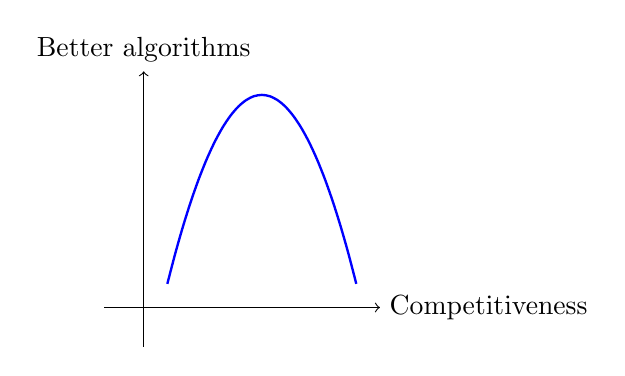
\begin{tikzpicture}
      \draw[->] (-.5,0) -- (3,0) node[right] {Competitiveness};
      \draw[->] (0,-.5) -- (0,3) node[above] {Better algorithms};
      \draw[scale=0.6,domain=0.5:4.5,smooth,variable=\x,blue, line width=0.3mm] plot ({\x},{4.5 - (\x - 2.5)^2});
      % \draw[scale=0.5,domain=-3:3,smooth,variable=\y,red]  plot ({\y*\y},{\y});
 \end{tikzpicture}

\caption{Inverted-U relationship between competitiveness and algorithms.}
\label{fig:inverted-U}
\end{center}
\end{figure}


\xhdr{Economic interpretation: the inverted-U relationship.}
Interpreting the adoption of better algorithms as ``innovation", our findings can be framed in terms of the inverted-U relationship between competition and innovation, as in Figure~\ref{fig:inverted-U}.%
\footnote{Here, ``innovation" refers to adoption of a better technology at a substantial R\&D expense to a given firm. It is not salient whether similar ideas and/or technologies already exist elsewhere. Adoption of exploration algorithms tends to require substantial R\&D effort in practice, even if the algorithms themselves are well-known in the research literature \citep[\eg see][]{DS-arxiv}.}
This is a well-established concept in the economics literature, dating back to \cite{Schumpeter-42}, whereby too little or too much competition is bad for innovation, but intermediate levels of competition tend to be better \citep[\eg][]{aghion2005competition,Vives-08}.

Our decision rules differ in terms of rationality: from fully rational decisions with \HardMax to relaxed rationality with \HardMaxRandom to an even more relaxed rationality with \SoftMaxRandom. The same distinctions also control the severity of competition between the principals: from cut-throat competition with \HardMax to a more relaxed competition with \HardMaxRandom, to an even more relaxed competition with \SoftMaxRandom. Indeed, with \HardMax you lose all customers as soon as you fall behind in performance, with \HardMaxRandom you get some small market share no matter what, and with \SoftMaxRandom you are further guaranteed a market share close to $\tfrac12$ as long as your performance is not much worse than the competition. The uniform choice among principals corresponds to no rationality and no competition. While agents' rationality and severity of competition are often modeled separately in the literature, it is not unusual to have them modeled with the same ``knob" \cite[\eg][]{Gabaix-16}.


We identify the inverted-U relationship driven by the rationality/competitiveness distinctions outlined above: from \HardMax to \HardMaxRandom to \SoftMaxRandom to \Uniform. We also find another, technically different, inverted-U relationship which zeroes in on the \HardMaxRandom model. We vary rationality/competitiveness inside this model, and track the marginal utility of switching to a better algorithm.

These inverted-U relationships are driven by different aspects in our model than the ones in the existing literature in economics. The latter focuses on the tradeoff between the R\&D costs and the benefits that the improved technology provides in the competition. In our case, the barriers for innovations arise entirely from the reputational consequences of exploration in competition, even in the absence of R\&D costs.

\ascomment{stopped here.}

\xhdr{Numerical simulations.}
We consider a basic frequentist model. We posit that the agents observe signals about the principals' past performance, and base their decisions on these signals alone, without invoking any prior knowledge or beliefs. The performance signals are abstracted and aggregated as a scalar \emph{reputation score} for each principal, modeled as a sliding window average of its rewards. Thus, agents' decision rule depends only on the two reputation scores. We refer to this variant as the \emph{\ExptsModel}.%
%\footnote{In comparison, the theoretical results focus on another extreme, with Bayesian rationality and no performance signals.}

We refine and expand the theoretical results in several ways.

\begin{itemize}
\item We compare \HardMax and \HardMaxRandom decision rules. We find that the greedy algorithm often wins under \HardMax, with a strong evidence of the ``death spiral" effect mentioned earlier.
 As predicted by the theory, better algorithms prevail if the expected number of ``random" users is sufficiently large. However, this effect is negligible for smaller parameter values.

%\footnote{\asedit{Reputation scores already introduce some noise into users' choices. However, the amount of noise due to this channel is typically small, both in our simulations and in practice, because reputation signals average over many datapoints.}}

\item We investigate the first-mover advantage as a different channel to vary the intensity of competition: from the first-mover to simultaneous arrival to late-arriver. (We focus on the \HardMax decision rule.) We find that the first-mover is incentivized to choose a more advanced exploration algorithm, whereas the late-arriver is often incentivized to choose the ``greedy algorithm" (more so than under simultaneous arrival). Consumer welfare is higher under early/late arrival than under simultaneous entry. We frame these results in terms of an inverted-U relationship.


%\footnote{\asedit{We consider the ``permanent monopoly" scenario for comparison only, without presenting any findings. We just assume that a monopolist chooses the greedy algorithm, because it is easier to deploy in practice. Implicitly, users have no ``outside option": the service provided is an improvement over not having it (and therefore the monopolist is not incentivized to deploy better learning algorithms). This is plausible with free ad-supported platforms such as Yelp or Google.}}

\item We investigate the algorithms' performance ``in isolation", \ie without competition. We suggest a new performance measure to explain why the greedy algorithm is sometimes not the best strategy under high levels of competition.\footnote{Note the discrepancy with our theoretical results on \HardMax: there, the greedy algorithm is always the best strategy, mainly because it is aware of the Bayesian prior (whereas in the simulations the prior is not available).}
     We find that mean reputation -- arguably, the most natural performance measure ``in isolation" -- is sometimes \emph{not} a good predictor for the outcomes under competition.

\item We decompose the first-mover advantage into two distinct effects: free data to learn from (\emph{data advantage}), and a more definite, and possibly better reputation compared to an entrant (\emph{reputation advantage}). We run additional experiments so as to isolate and compare these two effects. We find that either effect alone leads to a significant advantage under competition. The data advantage is larger than reputation advantage when the incumbent commits to a more advanced bandit algorithm. Finally, we find an ``amplification effect" of the data advantage: even a small amount thereof gets amplified under competition, causing a large difference in eventual market shares.

\end{itemize}

\ascomment{One downside of the story above: we may need to explain why we didn't simulate \SoftMaxRandom.}

\ascomment{The xhdr below is basically from Guy, with some rewordings by Alex.}

\xhdr{Economic interpretation: network effects of data.}
Our model speaks to policy discussions on regulating data-intensive digital platforms \citep{furman2019unlocking, scott2019committee}, and particularly to the ongoing debate on the role of data in the digital economy. One fundamental question in this debate is whether data can serve a similar role as traditional ``network effects", creating scenarios when only one firm can function in the market \citep{Rysman09, jullien2019economics}.
%whereby, when these effects are present, in many cases only one firm can function in the market, leading to competition \emph{for} the market being more important than competition \emph{in} the market \citep{Rysman09, jullien2019economics}.
The death spiral/amplification effects mentioned above have a similar flavor as network effects: a relatively small amount of exploration (resp., data advantage)  gets amplified under competition and causes the firm to be starved of users (resp., take over most of the market).
%\gaedit{We further find that a small data advantage for one firm gets amplified under competition and leads to that firm taking the entire market, showing that data can provide a similar incumbency advantage as those provided by traditional network effects and can serve as a barrier to entry in online markets.}
A distinctive feature of our approach is that we explicitly model the learning problem of the firms and consider them deploying algorithms for solving this problem.  Thus, we do not explicitly model the network effects, but they arise endogenously from our setup.

Our results highlight that understanding the performance of learning algorithms in isolation does not necessarily translate to understanding their impact in competition, precisely due to the fact that competition leads to the endogenous generation of data observed by the firms. Approaches such as \citet{lambrecht2015can, bajari2018impact, varian2018artificial} argue that the diminishing returns to scale and scope of data in isolation mitigate such data feedback loops,
%as non-existent
but ignore the differences induced by learning in isolation versus under competition. Furthermore, explicitly incorporating the interaction between learning technology and data creation allows us to speak on how data advantages are characterized and amplified not only by data quantity, but also the increased data quality gathered by better learning algorithms.

\ascomment{"Econ interpretation" xhdrs fit incely in "our results", as opposed to a separate subsection. Because: we can explain the "inverted-U" stuff right after "theory", before we put the simulation results on the stack. And the "network effects" stuff goes nicely right after the numerical results, without a big subsection break.}



\subsection{Further discussion}
\label{sec:discussion}

\xhdr{Significance.}
Our theory takes a basic Bayesian approach, a standard perspective in economic theory, and discovers several strong asymptotic results. The numerical simulations provide a more nuanced and ``non-asymptotic" perspective. In essence, we look for substantial effects within relevant time scales. In fact, we start our investigation by determining what time scales are relevant in the context of our model.

\ascomment{The next para makes a point that seems important (to me). Is this point clear?}

Our study has a dual purpose: (i) shed light on real-world implications of some typical scenarios, and (ii) investigate the space of models for describing the real world. As an example to clarify the latter point, consider the \HardMax model with simultaneous entry. It is is not necessarily the most realistic model, but arguably the most natural one to study \emph{a priori}. However, our results elucidate the need for more refined models that allow for ``free exploration" (\eg via random agents or early entry).

\xhdr{Modeling.}
Our models are stylized in several important  respects. Firms compete only on the quality of service, rather than, say, pricing or the range of products. Agents are myopic: they do not worry about how their actions impact their future utility.\footnote{In particular, agents do not attempt to learn over time, to second-guess or game future agents, or to manipulate the principals' learning algorithms. This is arguably typical in practice, in part because one agent's influence tends to be relatively small.}  Various performance signals available to the users, from personal experience to word-of-mouth to consumer reports, are abstracted as persistent ``reputation scores", and further simplified to average performance over a time window. On the machine learning side, our setup is geared to distinguish between ``simple" vs. ``better" vs. ``smart" bandit algorithms; we are not interested in state-of-art algorithms for very realistic bandit settings.

We consider two extremes: a simple Bayesian model with full Bayesian rationality and no performance signals, and a simple frequentist model with reputation scores and no prior knowledge or beliefs. For the theoretical results, the ``no-performance-signals" assumption makes agents' behavior independent of a particular realization of the prior. Therefore, we summarize each learning algorithm via its Bayesian-expected rewards, not worrying about its detailed performance on particular realizations of the prior.  Such summarization is essential for formulating lucid and general analytic results, let alone proving them. It is unclear how to incorporate performance signals in a theoretically tractable model. For the numerical results, the \ExptsModel accounts for competition in a more direct way \gaedit{by positing a more realistic model of consumer behavior that does not require them to have direct information on the algorithms deployed or the bandit problem faced by the firm. It further allows us to separate reputation vs. data advantage and makes our model amenable to numerical simulations.} Indeed, simulating the intricate interplay of learning dynamics and Bayesian priors appears computationally intractable.

\asedit{Principals' utilities (and, accordingly, bandit rewards) are not discounted with time.%
\footnote{However, our main theoretical result on the greedy algorithm extends to time-discounted rewards, see Section~\ref{sec:theory-extensions}.}
 While much of the early work focuses on  time-discounted bandits \citep{Gittins-book11}, non-discounted  formulations are prevalent in the bandits literature over the past two decades \citep{slivkins-MABbook,LS19bandit-book}, and better correspond to practical deployments \citep[\eg][]{DS-arxiv}. Moreover, the distinctions between better and worse bandit algorithms are not as well-understood under time-discounting.}

\gaedit{Finally, the assumption that firms commit to the algorithms at the start of the game deserves further justification. We impose this commitment assumption since it is more realistic than considering dynamic strategies and algorithms are, by definition, a commitment to a set of rules. In many contexts where such exploration algorithms are typically deployed, consumers arrive at such a rapid volume that it it is infeasible to consider a firm dynamically adapting its algorithm to each consumer that arrives. Indeed, \cite{DS-arxiv} points out how difficult it is to deploy standard exploration algorithms in practice and such dynamic strategies are substantially more difficult to deploy in practice. While it is possible to consider share-adaptive algorithms that would still keep the commitment assumption but allow for indirect dynamic responses to market conditions, such algorithms do not exist currently in the literature but are a good avenue for future work.}

\xhdr{Challenges.}
Much of the challenge in the theoretical results, both conceptual and technical, was in setting up the model and the theorems. Apart from zeroing in on the \TheoryModel, it was crucial to interpret the results and intuitions from the literature on multi-armed bandits so as to formulate meaningful and productive assumptions on bandit algorithms and Bayesian priors.

The numerical investigation is quite challenging even with a stylized model such as ours. An ``atomic experiment" is a competition game between a given pair of bandit algorithms, in a given competition model, on a given instance of a multi-armed bandit problem (and each such experiment is run many times to reduce variance).
Accordingly, we have a three-dimensional space of atomic experiments one needs to run and interpret: \{pairs of algorithms\} x \{competition models\} x \{bandit instances\}, and we are looking for findings that are consistent across this entire space. It is essential to keep each of the three dimensions small yet representative. In particular, we need to capture a huge variety of bandit instances with only a few representative examples. Further, we need a succinct and informative summarization of results within one atomic experiment and across multiple experiments (\eg see Table~\ref{sim_table}).


While amenable to simulations, the \ExptsModel appears difficult to analyze. This is for several reasons:
%
(i) intricate feedback loop from performance to reputations to users to performance;
%
(ii) mean reputation, most connected to our intuition, is sometimes a bad predictor in competition (see Sections~\ref{sec:isolation} and~\ref{sec:revisited}); and
%
(iii)
mathematical tools from regret-minimization would only produce ``asymptotic" results, which do not seem to suffice. Given the theoretical results on the \TheoryModel, and the fact that we are in the realm of stylized economic models, we believe that resolving first-order theoretical questions about the \ExptsModel would not add much value to this paper.



%%% Local Variables:
%%% mode: latex
%%% TeX-master: "main"
%%% End:


\section{Related work}
\label{sec:related-work}
Multi-armed bandits (\emph{MAB}) is a particularly elegant and tractable abstraction for tradeoff between \emph{exploration} and \emph{exploitation}: essentially, between acquisition and usage of information. MAB problems have been studied in Economics, Operations Research and Computer Science for many decades; see \citep{Bubeck-survey12,Gittins-book11,slivkins-MABbook} for background on regret-minimizing and Bayesian formulations, respectively. A discussion of industrial applications of MAB can be found in \citet{MWT-WhitePaper-2016}.

The literature on MAB is vast and multi-threaded. The most related
thread concerns regret-minimizing MAB formulations with IID rewards
\citep{Lai-Robbins-85,bandits-ucb1}. This thread includes ``smart" MAB
algorithms that combine exploration and exploitation, such as UCB1
\citep{bandits-ucb1} and Successive Elimination
\citep{EvenDar-icml06}, and ``naive'' MAB algorithms that separate
exploration and exploitation, including explore-first and
$\eps$-Greedy \citep[\eg see][]{slivkins-MABbook}.

The three-way tradeoff between exploration, exploitation and incentives has been studied in several other settings:
incentivizing exploration in a recommendation system
    \citep{Che-13,Frazier-ec14,Kremer-JPE14,ICexploration-ec15,Bimpikis-exploration-ms17,Bahar-ec16,ICexplorationGames-ec16-working},
dynamic auctions
    \cite[\eg][]{AtheySegal-econometrica13,DynPivot-econometrica10,Kakade-pivot-or13},
pay-per-click ad auctions with unknown click probabilities
    \cite[\eg][]{MechMAB-ec09,DevanurK09,Transform-ec10-jacm},
coordinating search and matching by self-interested agents
    \citep{Bobby-Glen-ec16},
as well as human computation
    \cite[\eg][]{RepeatedPA-ec14,Ghosh-itcs13,Krause-www13}.

\citet{Bolton-econometrica99,Keller-econometrica05,Johari-ec12} studied models with self-interested agents jointly performing exploration, with no principal to coordinate them.

There is a superficial similarity (in name only) between this paper and the line of work on ``dueling bandits"
    \citep[\eg][]{Yue-dueling12,Yue-dueling-icml09}.
The latter is not about competing bandit algorithms, but rather about scenarios where in each round two arms are chosen to be presented to a user, and the algorithm only observes which arm has ``won the duel".

Our setting is closely related to the ``dueling algorithms" framework \citep{DuelingAlgs-stoc11} which studies competition between two principals, each running an algorithm for the same problem. However, this work considers algorithms for offline / full input scenarios, whereas we focus on online machine learning and the explore-exploit-incentives tradeoff therein. Also, this work specifically assumes binary payoffs (\ie win or lose) for the principals.

\xhdr{Other related work in economics.} The competition vs. innovation relationship and the inverted-U shape thereof have been introduced in a classic book \citep{Schumpeter-42}, and remained an important theme in the literature ever since \cite[\eg][]{Aghion-QJE05,Vives-08}. Production costs aside, this literature treats innovation as a priori beneficial for the firm. Our setting is very different, as innovation in exploration algorithms may potentially hurt the firm.

A line of work on \emph{platform competition}, starting with \cite{Rysman09}, concerns competition between firms (\emph{platforms}) that improve as they attract more users (\emph{network effect}); see \citet{Weyl-White-14} for a recent survey. This literature is not concerned with \innovation, and typically models network effects exogenously, whereas in our model network effects are endogenous: they are created by MAB algorithms, an essential part of the model.

Relaxed versions of rationality similar to ours are found in several notable lines of work. For example, ``random agents" (a.k.a. noise traders) can side-step the ``no-trade theorem'' \citep{Milgrom-Stokey-82}, a famous impossibility result in financial economics. The \SoftMaxRandom model is closely related to the literature on \emph{product differentiation}, starting from \cite{Hotelling-29}, see \cite{Perloff-Salop-85} for a notable later paper.

There is a large literature on non-existence of equilibria due to small deviations   (which is related to the corresponding result for \HardMaxRandom), starting with \cite{Rothschild-Stiglitz-76} in the context of health insurance markets. Notable recent papers \citep{Veiga-Weyl-16,Azevedo-Gottlieb-17} emphasize the distinction between \HardMax and versions of \SoftMaxRandom.

% moved this thought to the intro.
\OMIT{While agents' rationality and severity of competition are often modeled separately in the literature, it is not unusual to have them modeled with the same ``knob" \cite[\eg][]{Gabaix-16}.}





%%% Local Variables:
%%% TeX-master: "main.tex"
%%% End: 


\section{Basic model and preliminaries}
\label{sec:model}
\xhdr{Principals and agents.} There are two principals and $T$ agents,
denoted, resp., principal $i\in \{1,2\}$ and agent $t\in [T]$. The game proceeds in (global) rounds. In each round $t\in [T]$, the following  interaction takes place. Agent $t$ arrives and chooses a principal $i_t\in \{1,2\}$. The principal chooses action $a_t\in A$, where $A$ is a fixed set of actions (same for both principals and all rounds).%
\footnote{We use `action' and `arm' interchangeably, as common in the literature on multi-armed bandits.}
The agent experiences this action and receives a reward $r_t\in \{ 0,1\}$ for this action, which is then observed by the principal. We posit \emph{stochastic rewards}: whenever a given action $a\in A$ is chosen, the reward is an independent draw from Bernoulli distribution with mean $\mu_a$. The mean rewards $\mu_a$ are fixed over time, and initially not known to anybody. The principals are completely unaware of the rounds when the opponent is chosen.

Thus, each principal follows the protocol of \emph{multi-armed bandits} (\emph{MAB}): in each round when it is chosen, it chooses an arm from $A$ and observes a reward for this action (and nothing else).

Each principal $i$ commits to an MAB algorithm \alg[i] before round $1$, and uses it throughout. The algorithm proceeds in time-steps:%
\footnote{These time-steps will sometimes be referred to as \emph{local steps/rounds}, so as to distinguish them from ``global rounds" defined before. We will omit the global vs. local distinction when clear from the context.} each time it is called, it outputs an arm from $A$, and inputs a reward for this action. The algorothm is called only in global rounds when principal $i$ is chosen.

\newcommand{\est}{\mathtt{EST}}

%\gaedit{\footnote{While our model assumes that agents have correct beliefs about the performance of the algorithms, only the beliefs themselves matter and so our results hold as long as all agents have the same initial beliefs, even if they are not aligned with the true prior.}}

\xhdr{Agents' response.} Each agent $t$ forms reward estimates $\est_i(t)\in [0,1]$ for each principal $i$, and uses them to choose the principal. Specifically, principal $1$ is chosen with probability
\begin{align}\label{eq:model-f}
p_t = \respF\rbr{ \est_1(t) - \est_2(t) },
\end{align}
where $\respF:[-1,1]\to [0,1]$ is the \emph{response function}, same for all agents. We assume that $\respF$ is monotonically non-decreasing, is larger than $\nicefrac12$ on the interval $(0,1]$, and smaller than $\nicefrac12$ on the interval $[-1,0)$. We consider three variants for $\respF$, depicted in  \reffig{fig:response-functions}:

\begin{figure}[t]
\begin{center}
  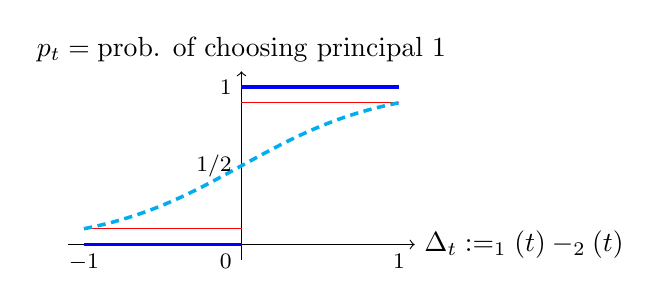
\begin{tikzpicture}[scale=2.0]
    \draw[->] (-1.1,0) -- (1.1,0) node[right]
    {$\Delta_t := \est_1(t) - \est_2(t)$};
    \draw[->] (0,-0.1) -- (0,1.1) node[above]
        {$p_t = \text{prob. of choosing principal 1}$};
    \draw[scale=1.0,domain=-1:0,smooth,variable=\q,blue, line width=0.50mm] plot ({\q},{0});
    \draw[scale=1.0,domain=0:1,smooth,variable=\q,blue,line width=0.50mm] plot ({\q},{1});
    \draw[scale=1.0,domain=-1:0,smooth,variable=\y,red]  plot ({\y},{0.1});
    \draw[scale=1.0,domain=0:1,smooth,variable=\y,red]  plot ({\y},{0.9});
    \draw[scale=1.0,domain=-1:1,smooth,variable=\y,cyan, line width=0.45mm, dash pattern=on 3pt off 2pt]  plot ({\y},{1/(1 + 1/(9^\y))});
    % \node[above, blue] at (0.5, 0.5) {\footnotesize $2 q (1 - q)$};
     \node[left] at (0, 0.5) {\footnotesize $1/2$};
     \node[left] at (0, 1) {\footnotesize $1$};
     \node[below left] at (0, 0) {\footnotesize $0$};
     \node[below ] at (1, 0) {\footnotesize $1$};
     \node[below ] at (-1, 0) {\footnotesize $-1$};
  \end{tikzpicture}
\end{center}
\caption{The three models for $\respF$: \HardMax is thick blue, \HardMaxRandom is red, and \SoftMaxRandom is dashed.}
\label{fig:response-functions}
\end{figure}

\begin{itemize}
\item \HardMax: $\respF$ equals $0$ on the interval $[-1,0)$ and $1$
  on the interval $(0,1]$. In words, a \HardMax agent
  deterministically chooses a principal with a higher reward estimate.

\item \HardMaxRandom:
    % $\respF$ equals $\eps$ on the interval $[-1,0)$ and $1-\eps'$ on the interval $(0,1]$, where $\eps,\eps'\in (0,\tfrac12)$ are some positive constants. In words, each agent is a \HardMax agent with probability $1-\eps-\eps'$, and with the remaining probability she makes a random choice.
    $\respF$ equals $\eps_0$ on the interval $[-1,0)$ and $1-\eps_0$ on the interval $(0,1]$, for some constant $\eps_0\in (0,\tfrac12)$. In words, each agent is a \HardMax agent with probability $1-2\eps_0$, and makes a random choice otherwise.


\item \SoftMaxRandom: $\respF$ lies in $[\eps_0,1-\eps_0]$, breaks ties fairly, and has a bounded derivative around $0$ (see Definition~\ref{def:SoftMax} for a formal definition).
\end{itemize}

\HardMaxRandom and \SoftMaxRandom can be seen as agent types that, resp., give some chance to the other principal and avoid sharp transitions in their probabilistic response. Alternatively, they can be realized as mixtures over more ``basic" agent types. Indeed, \HardMaxRandom is a mixture of \HardMax and ``random agents" (which choose a principal uniformly at random). One can obtain a \SoftMaxRandom response function using agent types that choose a principal $i$ with a largest reward estimate $\est_i$, unless $|\est_1-\est_2|$ is upper-bounded by some parameter $\theta$, in which case they choose uniformly. Then, we obtain \SoftMaxRandom as a mixture of random agents and these ``$\theta$-\HardMax'' agents, for a suitable distribution over $\theta$. \gaedit{We provide an interpretation of the ``random agents" as reputation-agnostic consumers that are not aware of or do not seek out the reputation signals available to them in the respective choice model variants.}

% \asedit{(We assume $\respF(-1)+\respF(1)=1$ in \HardMaxRandom and \SoftMaxRandom only to simplify notation.)}

%We say that $\respF$ is \emph{symmetric} if $\respF(-x)+\respF(x)=1$ for any $x\in [0,1]$. This implies \emph{fair tie-breaking}: $\respF(0)=\tfrac12$.

\xhdr{Bayesian vs. frequentist.}
We consider two model variants, Bayesian and frequentist. The main difference between the two concerns the agents' reward estimates $\est_i(t)$.

\begin{itemize}
\item In the \emph{\TheoryModel}, the mean reward vector $\mu = (\mu_a:\; a\in A)$ is drawn from a common Bayesian prior $\priorMu$. Each agent knows its global round $t$, but not the performance signals such as the current market shares. Agents' reward estimates are defined as posterior mean rewards:
        $\est_i(t) = \PMR_i(t) := \E\sbr{ r_t\mid i_t = i}$
    for each agent $t$ and principal $i$.%
\footnote{Formally, agents do the Bayesian update knowing $t$, the principals' algorithms, the prior $\priorMu$, and $\respF$.}

%Agents know the principals' algorithms.\gaedit{\footnote{While our model assumes that agents have correct beliefs about the performance of the algorithms, only the beliefs themselves matter and so our results hold as long as all agents have the same initial beliefs, even if they are not aligned with the true prior.}}

\item In the \emph{\ExptsModel}, agents' reward estimate for a given principal is the average reward of the last $M$ agents that chose this principal, interpreted as a current \emph{reputation score}. To make it meaningful initially, each principal enjoys a ``warm start": additional $T_0$ agents arrive before the game starts, and interact with the principal as described above.

\end{itemize}

\xhdr{Competition game.}
Some of our results explicitly study the game between the two principals, termed the \emph{competition game}. We model it as a simultaneous-move game: before the first agent arrives, each principal commits to an MAB algorithm.
Pure strategies in this game correspond to MAB algorithms.%
\footnote{Note that a mixed strategy is also a (randomized) MAB algorithm, \ie also a pure strategy.}
 Principal's utility is defined as the market share, \ie the number of agents that chose this principal. Principals are risk-neutral \gaedit{and aim to maximize their expected utility.}\gadelete{ : they optimize their expected utility.}


\xhdr{Extensions.} The \TheoryModel admits several extensions, detailed in Section~\ref{sec:theory-extensions}. First, all/most results extend to arbitrary reward distributions, allow reward-dependent utility, and carry over to a more general version of multi-armed bandits. Second, agents could have beliefs on $(\alg[1],\alg[2],\priorMu,\respF)$ that need not be correct; then, all results carry over with respect to these beliefs.
%Third, all results carry over \asmargincomment{check}  if each agent $t$ has a prior on her arrival time $t$, rather than know it exactly.
Third, we can handle a limited amount of non-stationarity in $\respF$ for the \HardMaxRandom and \SoftMaxRandom decision rules. Finally, the main result on \HardMax extends to time-discounted utilities.


\subsection{Discussion}
\label{sec:discussion}

Reflecting reality, we posit that the exploration strategies available to the principals are ``non-strategic" in nature. Even though the principals play a multi-step game, they do not react to each other's moves or to the agents' strategic choices. This is how industry approaches exploration algorithms, and for several good reasons. "Non-strategic" exploration is well-studied in machine learning, and yet it remains a very complex subject in research (as evidenced, \eg by the huge amount of activity therein). Even the seemingly simple algorithms are not straightforward to deploy in practice, and require a substantial investment in infrastructure \cite[\eg see the discussions in][]{DS-arxiv}. Responding to the competition represents another layer of complexity which has not been previously studied in this context, to the best of our knowledge, let alone made even remotely practical. Besides, the competitor's exploration strategy is typically not public, and understanding its exploration behavior via observations appears challenging even as a  research problem.%
\footnote{Principals could potentially react to the market share or (the difference in) reputation scores. However, baking these signals into one's exploration strategy runs the risk of over-interpreting our competition model, as they may change for exogenous reasons. Alternatively, one could use such signals, as well as the intuitions coming from this paper, to guide the platform's decisions regarding exploration.}


%\gaedit{Finally, the assumption that firms commit to the algorithms at the start of the game deserves further justification. We impose this commitment assumption since it is more realistic than considering dynamic strategies and algorithms are, by definition, a commitment to a set of rules. In many contexts where such exploration algorithms are typically deployed, consumers arrive at such a rapid volume that it it is infeasible to consider a firm dynamically adapting its algorithm to each consumer that arrives. Indeed, \cite{DS-arxiv} points out how difficult it is to deploy standard exploration algorithms in practice and such dynamic strategies are substantially more difficult to deploy in practice. While it is possible to consider share-adaptive algorithms that would still keep the commitment assumption but allow for indirect dynamic responses to market conditions, such algorithms do not exist currently in the literature but are a good avenue for future work.}



Our models are stylized in several important  respects. Firms compete only on the quality of service, rather than, say, pricing or the range of products. Agents are myopic: they do not worry about how their actions impact their future utility.\footnote{So, agents do not attempt to learn over time, second-guess or game future agents, or manipulate the principals' learning algorithms. This is arguably typical in practice, in part because one agent's influence tends to be small.}  Various performance signals available to the users, from personal experience to word-of-mouth to consumer reports, are abstracted as persistent ``reputation scores" reflecting the current reputation, and further simplified to average performance over a sliding time window.

We consider two extremes: a simple Bayesian model with full Bayesian rationality and no performance signals, and a simple frequentist model with reputation scores and no prior knowledge or beliefs. For the theoretical results, the ``no-performance-signals" assumption makes agents' behavior independent of a particular realization of the prior. Therefore, we summarize each learning algorithm via its Bayesian-expected rewards, not worrying about its detailed performance on particular realizations of the prior.  Such summarization is essential for formulating lucid and general analytic results, let alone proving them. It is unclear how to incorporate performance signals in a theoretically tractable model. For the numerical results, the \ExptsModel accounts for competition in a more direct way,
% \gaedit{by positing a more realistic model of consumer behavior that does not
not requiring users to have direct information on the algorithms deployed or the bandit problem faced by the firms. It further allows us to separate reputation vs. data advantage and makes our model amenable to numerical simulations.
%(Whereas simulating the intricate interplay of learning dynamics and Bayesian priors appears computationally intractable, see Footnote~\ref{fn:Tsquared}.)


On the machine learning side, our model captures big, qualitative differences between bandit algorithms, building on the well-established intuition in the literature. Comparisons between bandit algorithms are generally somewhat subtle, as some algorithms may be better for some problem instances and/or time intervals, and worse for some others. In particular, ``better" algorithms are better in the long run, but could be worse initially. We focus on a standard model of stochastic bandits. In Appendix~\ref{app:bg}, we present sufficient background on this model, accessible to non-specialists. However, we are less interested in state-of-art algorithms for realistic applications.

Bandit rewards are not discounted with time, reflecting the fact that non-discounted, regret-minimizing formulations has been prevalent in the bandits literature over the past two decades \citep{slivkins-MABbook,LS19bandit-book}, and better correspond to practical deployments \citep[\eg][]{DS-arxiv}. Also, the distinctions between better and worse bandit algorithms are not as well-understood under time-discounting.



\section{Full rationality (HardMax)}
\label{sec:rational}

In this section, we will consider the version in which
the agents are fully rational, in the sense that their response function is \HardMax. We show that principals are not incentivized to \emph{explore}--- \ie to deviate from \DynGreedy. The core technical result is that if one principal adopts \DynGreedy, then the other principal loses all agents as soon as he deviates.

To make this more precise, let us say that two MAB algorithms \emph{deviate} at (local) step $n$ if there is an action $a\in A$ and \asedit{a set of step-$n$ histories of positive probability such that any history $h$ in this set} is feasible for both algorithms, and under this history the two algorithms choose action $a$ with different probability.

\iffalse
\begin{definition}
  Suppose that an algorithm $\pi$ is not dynamic greedy. Then
  {\em the first exploration} for $\pi$ is the first time step where
  there is a non-zero probability that the recommended action has a
  lower expectation than exploitation option.\sw{define...}
\end{definition}
\fi


\begin{theorem}\label{thm:DG-dominance}
Assume \HardMax response function with fair tie-breaking. Assume that \alg[1] is \DynGreedy, and \alg[2] deviates from \DynGreedy starting from some (local) step $n_0<T$. Then all agents in global rounds $t\geq n_0$ select principal $1$.
\end{theorem}

\begin{corollary}\label{cor:DG-dominance}
The competition game between principals has a unique Nash equilibirium: both principals choose \DynGreedy.
\end{corollary}


\begin{remark}
This corollary holds under a more general model which allows time-discounting: namely, the utility of each principal $i$ in each global round $t$ is $U_{i,t}(r_t)$ if this principal is chosen, and $0$ otherwise, where $U_{i,t}(\cdot)$ is an arbitrary non-decreasing function with $U_{i,t}(0)>0$.
\end{remark}

\subsection{Proof of Theorem~\ref{thm:DG-dominance}}

The proof starts with two auxiliary lemmas: that deviating from \DynGreedy implies a strictly smaller Bayesian-expected reward, and that \HardMax implies a ``sudden-death" property: if one agent chooses principal $1$ with certainty, then so do all subsequent agents do. \asedit{We re-use both lemmas in later sections, so we state them in sufficient generality.}


\begin{lemma}\label{lm:DG-rew}
\asedit{Assume that \alg[1] is \DynGreedy, and \alg[2] deviates from \DynGreedy starting from some (local) step $n_0<T$. Then $\rew_1(n_0)>\rew_2(n_0)$. This holds for any response function $\respF$.}
\end{lemma}

\asedit{Lemma~\ref{lm:DG-rew} does not rely on any particular shape of the response function because it only considers the performance of each algorithm without competition.}

\begin{proof}[Proof of Lemma~\ref{lm:DG-rew}]
Since the two algorithms coincide on the first $n_0-1$ steps, it follows by symmetry that histories $H_{1,n_0}$ and $H_{2,n_0}$ have the same distribution. We use a \emph{coupling argument}: w.l.o.g., we assume the two histories coincide,
    $H_{1,n_0} = H_{2,n_0} = H$.

At local step $n_0$, \DynGreedy chooses an action $a_{1,n_0} = a_{1,n_0}(H)$
which maximizes the posterior mean reward given history $H$: for any realized history $h\in \support(H)$ and any action $a\in A$
\begin{align}\label{eq:lm:DG-rew-1}
 \PMR(a_{1,n_0} \mid H = h) \geq \PMR(a \mid H=h).
\end{align}

\ascomment{Rewrote the rest of the proof to account for positive-prob set of histories.}

By assumption \eqref{eq:assn-distinct}, it follows that 
\begin{align}\label{eq:lm:DG-rew-2}
 \PMR(a_{1,n_0} \mid H = h) > \PMR(a \mid H=h)
 \quad \text{for any $h\in \support(H)$ and $a\neq a_{1,n_0}(h)$.}
\end{align}

Since the two algorithms deviate at step $n_0$, there is a set $S\subset \support(H)$ of step-$n_0$ histories such that $\Pr[S]>0$ and any history $h\in S$ satisfies
    $\Pr[a_{2,n_0}\neq a_{1,n_0} \mid H=h]>0$.
Combining this with \eqref{eq:lm:DG-rew-2}, we deduce that 
\begin{align}\label{eq:lm:DG-rew-3}
 \PMR(a_{1,n_0} \mid H = h) > \E\left[ \mu_{a_{2,n_0}}\mid H=h \right]
 \quad\text{for each history $h\in S$}.
\end{align}
Using \eqref{eq:lm:DG-rew-1} and \eqref{eq:lm:DG-rew-3} and integrating over realized histories $h$, we obtain
    $\rew_1(n_0) > \rew_2(n_0)$.
\end{proof}


\begin{lemma}\label{lm:DG-sudden}
\asedit{Consider \HardMax response function with $\respF(0)\geq\tfrac12$.} 
Suppose \alg[1] is monotone, and $\PMR_1(t_0)>\PMR_2(t_0)$ for some global round $t_0$. Then $\PMR_1(t)>\PMR_2(t)$ for all subsequent rounds $t$.
\end{lemma}

\begin{proof}
Let us use induction on round $t\geq t_0$, with the base case $t=t_0$. Let $\mN=\mN_{1,t_0}$ be the agents' posterior distribution for $n_{1,t_0}$, the number of global rounds before $t_0$ in which principal $1$ is chosen. By induction, all agents from $t_0$ to $t-1$ chose principal $1$, so $\PMR_2(t_0)= \PMR_2(t)$. Therefore,
\[ \PMR_1(t)
    = \Ex{n\sim \mN}{\rew_1(n+1+t-t_0)}
    \geq \Ex{n\sim \mN}{\rew_1(n+1)}
    =\PMR_1(t_0) > \PMR_2(t_0)= \PMR_2(t), \]
where the first inequality holds because \alg[1] is monotone, and the second one is the base case.
\end{proof}

\begin{proof}[Proof of Theorem~\ref{thm:DG-dominance}]
Since the two algorithms coincide on the first $n_0-1$ steps, it follows by symmetry that $\rew_1(n) = \rew_2(n)$ for any $n< n_0$.
By Lemma~\ref{lm:DG-rew},
    $\rew_1(n_0) > \rew_2(n_0)$.

Recall that $n_i(t)$ is the number of global rounds $s<t$ in which principal $i$ is chosen, and $\posteriorN{i}{t}$ is the agents' posterior distribution for this quantity. By symmetry, each agent $t<n_0$ chooses a principal uniformly at random. It follows that
    $\posteriorN{1}{n_0} = \posteriorN{2}{n_0}$
(denote both distributions by $\mN$ for brevity), and $\mN(n_0-1)>0$.
Therefore:
\begin{align}
\PMR_1(n_0)
  &= \Ex{n\sim \mN} {\rew_1(n+ 1)}
   = \sum_{n = 0}^{n_0-1} \mN(n) \cdot{\rew_1(n + 1)} \nonumber \\
  & > \mN(n_0-1)\cdot {\rew_2(n_0)} + \sum_{n = 0}^{n_0-2}  \mN(n)\cdot{\rew_2(n + 1)}
    \nonumber \\
  &= \Ex{n\sim \mN}{\rew_2(n + 1)} = \PMR_2(n_0) \label{eq:pf:thm:DG-dominance}
\end{align}
So, agent $n_0$ chooses principal $1$. By Lemma~\ref{lm:DG-sudden} \asedit{(noting that \DynGreedy is monotone)}, all subsequent agents choose principal $1$, too.
\end{proof}


%\begin{theorem}
%  Suppose that the agents break ties uniformly at random, that is
%  $q=1/2$, then both principals playing \DynGreedy is the unique
%  equilibrium.
%\end{theorem}
%
%\begin{proof}
%  Suppose that both principals play dynamic greedy. The result
%  of Theorem~\ref{thm:DG-dominance} shows that there is no beneficial deviation
%  for both principals, so this forms a pure strategy equilibrium.
%
%  Now we will show that no other strategy profile can form equilibrium
%  in this game.  Suppose that both principals play some mixed
%  strategies that places non-zero probability on algorithms other than
%  dynamic greedy. We know one of the principals $p_j$ is getting no
%  more than $T/2$ agents in expectation. If $p_j$ switch to playing
%  only dynamic greedy, he can get strictly more than $T/2$ agents
%  by Theorem~\ref{thm:DG-dominance}. Thus, such a strategy profile will not form
%  an equilibrium.  Finally, suppose that $p_1$ plays dynamic greedy
%  and $p_2$ plays algorithms other than dynamic greedy with non-zero
%  probability. By Theorem~\ref{thm:DG-dominance}, we know that $p_2$ gets less
%  than $T/2$ agents in expectation. This means switching to dynamic
%  greedy will strictly improve the expected utility to $T/2$, so such
%  strategy profile cannot form an equilibrium either.
%\end{proof}


\subsection{\HardMax with biased tie-breaking}
\label{sec:HardMax-biased}

The \HardMax model is very sensitive to the tie-breaking rule. For starters, if ties are  broken deterministically in favor of principal $1$, then principal 1 can get all agents no matter what the other principal does, simply by using \StaticGreedy.

\begin{theorem}\label{thm:HardMax-hardTies}
Assume \HardMax response function with $\respF(0)=1$ (ties are always broken in favor of principal $1$). If \alg[1] is \StaticGreedy, then all agents choose principal $1$.
\end{theorem}

\begin{proof}
Agent $1$ chooses principal $1$ because of the tie-breaking rule. Since \StaticGreedy is trivially monotone, all the subsequent agents choose principal $1$ by an induction argument similar to the one in the proof of Lemma~\ref{lm:DG-sudden}.
\end{proof}

A more challenging scenario is when the tie-breaking is biased in favor of principal 1, but not deterministically so: $\respF(0)>\tfrac12$. Then this principal also has a ``winning strategy" no matter what the other principal does. Specifically, principal 1 can get all but the first few agents, under a mild technical assumption that \DynGreedy deviates from \StaticGreedy. Principal 1 can use \DynGreedy, or any other monotone MAB algorithm that coincides with \DynGreedy in the first few steps.

%We can generalize the theorem top the case of $q >1/2$ if the
%principal $p_1$ can guarantee better than the a priori best action to
%all the agents following the second.


\begin{theorem}\label{thm:HardMax-biased}
Assume \HardMax response function with $\respF(0)>\tfrac12$ (\ie tie-breaking is biased in favor of principal $1$). Assume the prior $\mP$ is such that \DynGreedy deviates from \StaticGreedy starting from some step $n_0$. Suppose that principal $1$ runs a monotone MAB algorithm that coincides with \DynGreedy in the first $n_0$ steps. Then all agents $t\geq n_0$ choose principal $1$.
\end{theorem}


\begin{proof}
The proof re-uses Lemmas~\ref{lm:DG-rew} and~\ref{lm:DG-sudden}, which do not rely on fair tie-breaking.

Because of the biased tie-breaking, for each global round $t$ we have:
\begin{align}\label{eq:thm:HardMax-biased-PMRtoPr}
\text{if $\PMR_1(t)\geq \PMR_2(t)$ then $\Pr[i_t=1]>\tfrac12$.}
\end{align}
Recall that $i_t$ is the principal chosen in global round $t$.

Let $m_0$ be the first step when \alg[2] deviates from \DynGreedy, or \DynGreedy deviates from \StaticGreedy, whichever comes sooner. \asedit{Then \alg[2], \DynGreedy and \StaticGreedy coincide on the first $m_0-1$ steps. Moreover, $m_0\leq n_0$ (since \DynGreedy deviates from \StaticGreedy at step $n_0$), so \alg[1] coincides with \DynGreedy on the first $m_0$ steps.

So, $\rew_1(n)=\rew_2(n)$ for each step $n<m_0$, because \alg[1] and \alg[2] coincide on the first $m_0-1$ steps. Moreover, if \alg[2] deviates from \DynGreedy at step $m_0$ then
    $\rew_1(m_0) > \rew_2(m_0)$ 
by Lemma~\ref{lm:DG-rew}; else, we trivially have
    $\rew_1(m_0) = \rew_2(m_0)$.} To summarize:
\begin{align}\label{eq:thm:HardMax-biased-rew}
    \rew_1(n)\geq\rew_2(n)\quad \text{for all steps $n\leq m_0$}.
\end{align}

We claim that $\Pr[i_t=1]>\tfrac12$ for all global rounds $t\leq m_0$. We prove this claim using induction on $t$. The base case $t=1$ holds by \eqref{eq:thm:HardMax-biased-PMRtoPr} and the fact that in step 1, \DynGreedy chooses the arm with the highest prior mean reward. For the induction step, we assume that $\Pr[i_t=1]>\tfrac12$ for all global rounds $t<t_0$, for some $t_0\leq  m_0$. It follows that distribution $\posteriorN{1}{t_0}$ stochastically dominates distribution $\posteriorN{2}{t_0}$.%
\footnote{For random variables $X,Y$ on \R, we say that $X$ \emph{stochastically dominates} $Y$ if $\Pr[X\geq x] \geq \Pr[Y\geq x]$ for any $x\in \R$.}
Observe that
\begin{align}\label{eq:thm:HardMax-biased-PMR-aux}
\PMR_1(t_0)
  = \Ex{n\sim \posteriorN{1}{t_0}} {\rew_1(n+1)}
  \geq \Ex{n\sim \posteriorN{2}{t_0}} {\rew_2(n+1)}
  = \PMR_2(t_0).
\end{align}
So the induction step follows by \eqref{eq:thm:HardMax-biased-PMRtoPr}. Claim proved.

Now let us focus on global round $m_0$, and denote $\mN_i = \posteriorN{i}{m_0}$.  By the above claim,
\begin{align}\label{eq:thm:HardMax-biased-mN}
\text{$\mN_1$ stochastically dominates $\mN_2$, and moreover
    $\mN_i(m_0-1)>\mN_i(m_0-1)$.}
\end{align}

By definition of $m_0$, either (i) \alg[2] deviates from \DynGreedy starting from local step $m_0$, which implies $\rew_1(m_0)> \rew_2(m_0)$ by Lemma~\ref{lm:DG-rew}, or (ii) \DynGreedy deviates from \StaticGreedy starting from local step $m_0$, which implies $\rew_1(m_0)>\rew_1(m_0-1)$ by Lemma~\ref{dgmono}. In both cases, using \eqref{eq:thm:HardMax-biased-rew} and \eqref{eq:thm:HardMax-biased-mN}, it follows that the inequality in \eqref{eq:thm:HardMax-biased-PMR-aux} is strict for $t_0=m_0$.

Therefore, agent $m_0$ chooses principal $1$, and by Lemma~\ref{lm:DG-sudden} so do all subsequent agents.
\end{proof}


% OLD PROOF (assuming alg1 coincides with DG on first two rounds, etc.
% We consider two cases, depending on the arm $a_{2,1}$ that principal $2$ chooses in the same step. The interesting case is $a_{2,1}=1$.
%Then agent $1$ selects principal $1$ with probability $q:=\respF(0)>\tfrac12$. Therefore, agent $2$ forms the following posterior mean rewards:
%\begin{align*}
%  \PMR_1(2) &= (1-q)\cdot \E[\mu_1] + q\cdot \rew_1(2)
%    \EqComment{for principal 1}\\
%  \PMR_2(2) &= q\cdot \E[\mu_1] + (1-q)\cdot \rew_2(2)
%    \EqComment{for principal 2}.
%\end{align*}
%We know that
%    $\rew_1(2) > \E[\mu_1]$
%(\DynGreedy is strictly monotone in the first $2$ rounds)
%from Lemma~\ref{dgmono}, and
%    $\rew_1(2) \geq \rew_2(2)$
%by Lemma~\ref{lm:DG-rew}. It follows that
%    $\PMR_1(2)>\PMR_2(2)$,
%and consequently agent $2$ chooses principal $1$. The subsequent agents choose principal $1$ by Lemma~\ref{lm:DG-sudden}.
%
%The remaining case is $a_{2,1}\neq 1$: principal $p_2$ does not recommend arm $1$ in the first step. Since all other arms have a strictly lower prior mean reward, agent $1$ chooses principal $1$. The subsequent agents choose principal $1$ by Lemma~\ref{lm:DG-sudden}.



% \begin{lemma}
%   Let $\mu^2_{DG}$ the expected reward of action of \DynGreedy
%   in the second step. Then $\mu^2_{DG} > \mu_1$.
% \end{lemma}

% \begin{proof}
%   \sw{todo. This requires an assumption that the second arm has
%     non-zero probability of beating the first one.}
% \end{proof}



% Steven's proof for a more general version with alg1 = BIC algo
%Agent $1$ chooses principal $1$ because of the tie-breaking rule,
%  Since principal $p_1$ in the first step recommends arm 1, the agent
%  selects principal $p_1$ (due to the tie breaking rule).  Agent $2$
%  knows that agent $1$ selected $p_1$. Because of BIC, she knows $p_1$
%  will offer reward no lower than $p_2$ in expectation.  By induction,
%  all the agents select principal $p_1$.



%\sw{We also have an observation saying if one principal starts with a
%  better dynamic greedy will just dominate the game. It could do some
%  amount of exploration while having better Bayesian per-round regret
%  than the other principal. This means the other principal will never
%  have any agents arriving for learning.}

%%% Local Variables:
%%% TeX-master: "main.tex"
%%% End: 

\section{Relaxed rationality: HardMax \& Random}
\label{sec:random}
This section is dedicated to the \HardMaxRandom response model, where each principal is always chosen with some positive baseline probability. The main technical result for this model states that a principal with asymptotically better \BIR wins by a large margin: after a ``learning phase" of constant duration, all agents choose this principal with maximal possible probability $\respF(1)$. For example, a principal with $\BIR(n)\leq \tilde{O}(n^{-1/2})$ wins over a principal with $\BIR(n)\geq \Omega(n^{-1/3})$. However, this positive result comes with a significant caveat detailed in Section~\ref{sec:random-greedy}.

We formulate and prove a cleaner version of the result, followed by a more general formulation developed in a subsequent Remark~\ref{rem:random-messy}. We need to express a property that \alg[1] eventually catches up and surpasses \alg[2], even if initially it receives only a fraction of traffic. For the cleaner version, we assume that both algorithms are well-defined for an infinite time horizon, so that their \BIR does not depend on the time horizon $T$ of the game.  Then this property can be formalized as:
\begin{align}\label{eq:random-better-clean}
(\forall \eps>0)\qquad
\BIR_1(\eps n)/\BIR_2(n) \to 0.
\end{align}
In fact, a weaker version of \eqref{eq:random-better-clean} suffices:
denoting $\eps_0 = \respF(-1)$, for some constant $n_0$ we have
\begin{align}\label{eq:random-better-weaker}
(\forall n\geq n_0) \qquad
\BIR_1(\eps_0 n/2)/\BIR_2(n) <\tfrac12.
\end{align}
We also need a very mild technical assumption on the ``bad" algorithm:
\begin{align}\label{eq:random-assn}
 (\forall n\geq n_0) \qquad
  \BIR_2(n) > 4\,e^{-\eps_0 n/12}.
\end{align}

\begin{theorem}\label{thm:random-clean}
Assume \HardMaxRandom response function. Suppose both algorithms are monotone and well-defined for an infinite time horizon, and satisfy~\eqref{eq:random-better-weaker} and~\eqref{eq:random-assn}. Then each agent $t\geq n_0$ chooses principal $1$ with maximal possible probability $\respF(1) = 1- \eps_0$.
\end{theorem}

\begin{proof}
Consider global round $t\geq n_0$. Recall that each agent chooses principal $1$ with probability at least
    $\respF(-1)>0$.

Then
    $\E[n_1(t+1)] \geq 2\eps_0\,t $.
By Chernoff Bounds (Theorem~\ref{thm:chernoff}), we have that
    $n_1(t+1)\geq \eps_0 t$
holds with probability at least $1-q$,
where $q = \exp(-\eps_0 t/12)$.

We need to prove that
    $\PMR_1(t) - \PMR_2(t)>0$.
For any $m_1$ and $m_2$, consider the quantity
\[ \Delta(m_1,m_2) := \BIR_2(m_2+1) - \BIR_1(m_1+1).\]
Whenever $m_1 \geq \eps_0 t/2 -1$ and $m_2<t$, it holds that
\begin{align*}
\Delta(m_1,m_2) \geq \Delta(\eps_0 t / 2, t)
    \geq \BIR_2(t)/2.
\end{align*}
The above inequalities follow, resp., from algorithms' monotonicity and \eqref{eq:random-better-weaker}. Now,
\begin{align*}
\PMR_1(t) - \PMR_2(t)
    &= \Ex{m_1\sim \posteriorN{1}{t},\;m_2\sim \posteriorN{2}{t}}{\Delta(m_1,m_2)} \\
    &\geq -q
        + \Ex{m_1\sim \posteriorN{1}{t},\;m_2\sim \posteriorN{2}{t}}
            {\Delta(m_1,m_2)\mid m_1 \geq \eps_0 t/2-1} \\
    &\geq \BIR_2(t)/2-q \\
    &> \BIR_2(t)/4 > 0  \EqComment{by \eqref{eq:random-assn}}. \qedhere
\end{align*}
\end{proof}

\begin{remark}\label{rem:random-messy}
  Many standard MAB algorithms in the literature are parameterized by
  the time horizon $T$. Regret bounds for such algorithms usually
  include a polylogarithmic dependence on $T$. In particular, a
  typical upper bound for \BIR has the following form:
  \OMIT{\footnote{We
    provide upper bounds on \BIR for several standard MAB algorithms
    to illustrate these dependencies in the appendix.\sw{added}}}
\begin{align}
    \BIR(n\mid T)\leq \polylog(T)\cdot n^{-\gamma}
    \quad \text{for some $\gamma\in(0,\tfrac12]$}.
\end{align}
Here we write $\BIR(n\mid T)$ to emphasize the dependence on $T$.

We generalize \eqref{eq:random-better-weaker} to handle the dependence
on $T$: there exists a number $T_0$ and a function $n_0(T)\in \polylog(T)$ 
such that 
\begin{align}\label{eq:random-better-messy}
(\forall T\geq T_0,\; n\geq n_0(T)) \quad
\frac{\BIR_1(\eps_0 n /2\mid T)}{\BIR_2(n\mid T)} <\frac12.
\end{align}
If this holds, we say that \alg[1] \emph{BIR-dominates} \alg[2].

We provide a version of Theorem~\ref{thm:random-clean} in which algorithms are parameterized with time horizon $T$ and condition \eqref{eq:random-better-weaker} is replaced with \eqref{eq:random-better-messy}; its proof is very similar and is omitted.
\end{remark}

%\begin{theorem}\label{thm:random-messy}
%Assume \HardMaxRandom response function, and algorithms that satisfy \eqref{eq:random-better-messy} and~\eqref{eq:random-assn}. Then each agent
%    $t\geq n_0(T)$ chooses principal $1$ with probability $\respF(1)$.
%\end{theorem}


%Let \alg be a monotone MAB algorithm and $\mA$ be a finite set of monotone MAB algorithms such that each algorithm in $\mA$ satisfies \eqref{eq:random-assn} and is ``dominated" by \alg in the sense of \eqref{eq:random-better-messy}.
%Assume principals can only choose algorithms from $\mA\cup \{\alg\}$.

To state a game-theoretic corollary of Theorem~\ref{thm:random-clean}, we consider a version of the competition game between the two principals in which they can only choose from a finite set $\mA$ of monotone MAB algorithms. One of these algorithms is ``better" than all others; we call it the \emph{special} algorithm. Unless specified otherwise, it BIR-dominates all other allowed algorithms. The other algorithms satisfy \eqref{eq:random-assn}. We call this game the \emph{restricted competition game}.

\begin{corollary}\label{cor:random}
Assume \HardMaxRandom response function. Consider the restricted competition game with special algorithm \alg. Then, for any sufficiently large time horizon $T$, this game has a unique Nash equilibrium: both principals choose \alg.
\end{corollary}


\subsection{A little greedy goes a long way}
\label{sec:random-greedy}

Given any monotone MAB algorithm other than \DynGreedy, we design a modified algorithm which learns at a slower rate, yet ``wins the game" in the sense of Theorem~\ref{thm:random-clean}. As a corollary, the competition game with unrestricted choice of algorithms typically does not have a Nash equilibrium.

Given an algorithm \alg[1] that deviates from \DynGreedy starting from
step $n_0$ and a ``mixing'' parameter $p$, we will construct a
modified algorithm as follows.
\begin{enumerate}
\item The modified algorithm coincides with \alg[1] (and \DynGreedy)
for the first $n_0-1$ steps;
\item In each step $n\geq n_0$, \alg[1] is invoked with probability
  $1-p$, and with the remaining probability $p$ does the ``greedy
  choice": chooses an action with the largest posterior mean reward
  given the current information collected by \alg[1].
\end{enumerate}
%The modified algorithm is called \emph{greedy deviation}, with probability parameter $p$.
For a cleaner comparison between the two algorithms, the modified algorithm does not record rewards received in steps with the ``greedy choice". Parameter $p>0$ is the same for all steps. We state the main result and defer the detailed proof to the appendix.

\begin{theorem}\label{thm:random-greedy}
Assume symmetric \HardMaxRandom response function. Let $\eps_0 = \respF(-1)$ be the baseline probability. Suppose \alg[1] deviates from \DynGreedy starting from some step $n_0$. Let \alg[2] be the modified algorithm, as described above, with mixing parameter $p$ such that
    $(1-\eps_0)(1-p)>\eps_0$.
Then each agent $t\geq n_0$ chooses principal $2$ with maximal possible probability $1-\eps_0$.
\end{theorem}

\begin{corollary}\label{cor:random-greedy}
  Suppose that both principals can choose any monotone MAB algorithm, and assume the symmetric \HardMaxRandom response
  function. Then for any time
  horizon $T$, the only possible \emph{pure} Nash equilibrium is one
  where both principals choose \DynGreedy. Moreover, no pure Nash
  equilibrium exists when some algorithm ``dominates" \DynGreedy in
  the sense of \eqref{eq:random-better-messy} and the time horizon $T$
  is sufficiently large.
\end{corollary}


\begin{remark}
The modified algorithm performs exploration % ingests information
at a slower rate. Let us argue how this may translate  into a larger \BIR compared to the original algorithm. Let  $\BIR'_1(n)$ be the \BIR of the ``greedy choice" after after $n-1$ steps of \alg[1]. Then
\begin{align}\label{eq:random-BIR}
\BIR_2(n)
    &= \Ex{m\sim (n_0-1)+\term{Binomial}(n-n_0+1,1-p)}{(1-p) \cdot \BIR_1(m) + p \cdot \BIR'_1(m)}.
\end{align}
In this expression, $m$ is the number of times \alg[1] is invoked in the first $n$ steps of the modified algorithm. Note that
    $\E[m] = n_0-1 + (n-n_0+1)(1-p) \geq (1-p)n$.

Suppose $\BIR_1(n)= \beta n^{-\gamma}$ for some constants $\beta,\gamma>0$. Further, assume 
    $\BIR'_1(n)\geq  c\; \BIR_1(n)$,
for some $c>1-\gamma$.
Then for all $n\geq n_0$ and small enough $p>0$ it holds that:
\begin{align*}
 \BIR_2(n) 
    &\geq  (1-p+pc)\; \E[\; \BIR_1(m) \;] \\
\E[\; \BIR_1(m) \;]
    &\geq \BIR_1(\; \E[m] \;) &\qquad\text{(By Jensen's inequality)} \\
    &\geq \BIR_1(\; (1-p)n \;) &\qquad\text{(since $\E[m]\geq n(1-p)$)}  \\
    &\geq \beta\cdot n^{-\gamma} \cdot (1-p)^{-\gamma} 
        &\qquad\text{(plugging in $\BIR_1(n)=\beta n^{-\gamma}$)}  \\
    &> \BIR_1(n)\;\; (1-p\gamma)^{-1}
        &\qquad\text{(since $(1-p)^\gamma < 1-p\gamma$)}.\\
\BIR_2(n) 
    &>\alpha\cdot \BIR_1(n),
    &\text{where} \quad 
    \alpha = \tfrac{1-p+pc}{1-p\gamma}>1.
\end{align*}
(In the above equations, all expectations are over $m$ distributed as in \eqref{eq:random-BIR}.)
\end{remark}

%%% Local Variables:
%%% TeX-master: "main.tex"
%%% End: 

\section{SoftMax response function}
\label{sec:soft}
This section is devoted to the \SoftMaxRandom model. We recover a positive result under the assumptions from Theorem~\ref{thm:random-clean} (albeit with a weaker conclusion), and then proceed to a much more challenging result under weaker assumptions. We start with a formal definition:

\begin{definition}\label{def:SoftMax}
A response function $\respF$ is \SoftMaxRandom if the following conditions hold:
\begin{OneLiners}
\item  $\respF(\cdot)$ is bounded away from $0$ and $1$:
    $\respF(\cdot)\in [\eps,1-\eps]$ for some $\eps\in (0,\tfrac12)$,
\item  the response function
 $\respF(\cdot)$ is ``smooth" around $0$:
 \begin{align}\label{eq:SoftMax-smooth}
 \exists\, \text{constants $\delta_0,c_0,c'_0>0$}
    \qquad \forall x\in [-\delta_0,\delta_0] \qquad
    c_0 \leq \respF'(x) \leq c'_0.
 \end{align}
\item fair tie-breaking: $\respF(0)=\tfrac12$.
\end{OneLiners}
\end{definition}

\begin{remark}
\asedit{This definition is fruitful when parameters $c_0$ and $c_0'$ are close to $\tfrac12$. Throughout, we assume that \alg[1] is better than \alg[2], and obtain results parameterized by $c_0$. By symmetry, one could assume that \alg[2] is better than \alg[1], and obtain similar results parameterized by $c_0'$.}
\end{remark}

Our first result is a version of Theorem~\ref{thm:random-clean}, with the same assumptions about the algorithms and essentially the same proof. The conclusion is much weaker: we can only guarantee that each agent $t\geq n_0$ chooses principal 1 with probability slightly larger than $\tfrac12$. This is essentially unavoidable in a typical case when both algorithms satisfy $\BIR(n)\to 0$, by Definition~\ref{def:SoftMax}.

\begin{theorem}\label{thm:SoftMax-weak}
  Assume \SoftMaxRandom response function. Suppose \alg[1] has better
  \BIR in the sense of \eqref{eq:random-better-weaker}, and \alg[2]
  satisfies the condition \eqref{eq:random-assn}. Then each agent
  $t\geq n_0$ chooses principal $1$ with probability
\begin{align}\label{eq:thm:SoftMax-weak}
     \Pr[i_t = 1]\geq \tfrac12 +  \tfrac{c_0}{4}\; \BIR_2(t).
\end{align}
\end{theorem}

\begin{proof}[Proof Sketch]
We follow the steps in the proof of Theorem~\ref{thm:random-clean} to derive \begin{align*}
\PMR_1(t) - \PMR_2(t)
    &\geq \BIR_2(t)/2 -q,
    \quad \text{where $q = \exp(-\eps_0 t/12)$.}
\end{align*}
This is at least $\BIR_2(t)/4$ by \eqref{eq:random-assn}. Then \eqref{eq:thm:SoftMax-weak} follows by the smoothness condition \eqref{eq:SoftMax-smooth}.
\end{proof}

\newcommand{\BReg}{\term{BReg}}

We recover a version of Corollary~\ref{cor:random}, if each principal's utility is the number of users (rather than the more general model in \eqref{eq:general-utility}). We also need a mild technical assumption that cumulative Bayesian regret (\BReg) tends to infinity. \BReg is a standard notion from the literature (along with \BIR):
\begin{align}\label{eq:SoftMax-BReg}
\BReg(n) := n\cdot \E_{\mu\sim\priorMu}
    \left[ \max_{a\in A} \mu_a\right] - \sum_{n=1}^n \rew(n')
    = \sum_{n'=1}^n \BIR(n').
\end{align}

\begin{corollary}\label{cor:SoftMax}
Assume that the response function is \SoftMaxRandom, and each principal's  utility is the number of users.
%
%Suppose principals can only choose algorithms from $\mA\cup \{\alg\}$, where $\mA\cup \{\alg\}$ is a finite set of monotone MAB algorithms such that each algorithm in $\mA$ satisfies \eqref{eq:random-assn} and $\BReg(n)\to \infty$, and is ``dominated" by \alg in the sense of \eqref{eq:random-better-messy}.
%
Consider the restricted competition game with special algorithm \alg, and assume that all other allowed algorithms satisfy $\BReg(n)\to \infty$. Then, for any sufficiently large time horizon $T$, this game has a unique Nash equilibrium: both principals choose \alg.
\end{corollary}

Further, we prove a much more challenging result in which the
condition \eqref{eq:random-better-weaker} is replaced with a much
weaker ``BIR-dominance'' condition. For clarity, we will again assume
that both algorithms are well-defined for an infinite time
horizon. The \emph{weak BIR dominance} condition says there exist
constants $\beta_0, \alpha_0\in (0, 1/2)$ and $n_0$ such that
 \begin{align}\label{eq:SoftMax-better}
   (\forall n\geq n_0) \quad
   \frac{\BIR_1((1-\beta_0)\, n)}{\BIR_2(n)} <1-\alpha_0.
 \end{align}
% for some $n_0(T)\in \polylog(T)$ and constants
% $\beta_0,\alpha_0\in (0, 1/2)$,
% \begin{align}\label{eq:SoftMax-better}
% (\forall n\geq n_0(T)) \quad
% \frac{\BIR_1((1-\beta_0)\, n\mid T)}{\BIR_2(n\mid T)} <1-\alpha_0.
% \end{align}
 If this holds, we say that \alg[1] \emph{weakly BIR-dominates}
 \alg[2]. Note that the condition \eqref{eq:random-better-messy}
 involves sufficiently small multiplicative factors (resp., $\eps_0/2$
 and $\tfrac12$), the new condition replaces them with factors that
 can be arbitrarily close to $1$.

 We make a mild assumption on \alg[1] that its $\BIR_1(n)$ tends to
 0. Formally, for any $\eps > 0$, there exists some $n(\eps)$ such
 that
 \begin{align}\label{eq:so-mild}
   (\forall n\geq n(\eps)) \qquad \BIR_1(n) \leq \eps.
 \end{align}
 We also require a slightly stronger version of the technical
 assumption~\eqref{eq:random-assn}:%  for any $\eps > 0$, there exists
 % $n(\eps)$ such that for
for some $n_0$,
\begin{align}\label{eq:SoftMax-assn-strong}
 % (\forall n\geq n(\eps)) \qquad
 %  \BIR_2(n) > e^{-\eps n}. %used to be 4exp( -\eps n/6)
(\forall n\geq n_0) \qquad 
\BIR_2(n) \geq \frac{4}{\alpha_0} \exp \left( \frac{-\min\{\eps_0, 1/8\} n}{12}\right)
\end{align}




\begin{theorem}\label{thm:SoftMax-strong}
  Assume the \SoftMaxRandom response function. Suppose \alg[1]
  weakly-BIR-dominates \alg[2], \alg[1] satisfies \eqref{eq:so-mild},
  and \alg[2] satisfies \eqref{eq:SoftMax-assn-strong}. Then there
  exists some $t_0$ such that each agent $t\geq t_0$ chooses principal
  $1$ with probability
\begin{align}\label{eq:thm:SoftMax-strong}
     \Pr[i_t = 1]\geq \tfrac12 +  \tfrac{c_0\alpha_0}{4}\; \BIR_2(t).
\end{align}
\end{theorem}




The main idea behind our proof is that even though \alg[1] may have a
slower rate of learning in the beginning, it will gradually catch up
and surpass \alg[2]. We will describe this process in two phases. In
the first phase, \alg[1] receives a random agent with probability at
least $\respF(-1) = \eps_0$ in each round. Since $\BIR_1$ tends to 0,
the difference in \BIR{s} between the two algorithms is also
diminishing. Due to the \SoftMaxRandom response function, \alg[1]
attracts each agent with probability at least $1/2 - O(\beta_0)$ after
a sufficient number of rounds. Then the game enters the second phase:
both algorithms receive agents at a rate close to $\tfrac12$, and the
fractions of agents received by both algorithms --- $n_1(t)/t$ and
$n_2(t)/t$ --- also converge to $\tfrac12$. At the end of the second
phase and in each global round afterwards, the counts $n_1(t)$ and
$n_2(t)$ satisfy the weak BIR-dominance condition, in the sense that
they both are larger than $n_0$ and $n_1(t)\geq (1-\beta_0)\; n_2(t)$.
At this point, \alg[1] actually has smaller $\BIR$, which reflected in the {\PMR}s eventually. Accordingly, from then on \alg[1]
attracts agents at a rate slightly larger than $\tfrac12$. We prove
that the ``bump'' over $\tfrac12$ is at least on the order of
$\BIR_2(t)$.


\begin{proof}[Proof of Theorem~\ref{thm:SoftMax-strong}]
  Let $\beta_1 = \min\{c_0'\delta_0, \beta_0/20\}$ with $\delta_0$
  defined in~\eqref{eq:SoftMax-smooth}.  Recall each agent chooses
  \alg[1] with probability at least $\respF(-1)= \eps_0$.  By
  condition \eqref{eq:so-mild} and \eqref{eq:SoftMax-assn-strong},
  there exists some sufficiently large $T_1$ such that for any
  $t\geq T_1$, $\BIR_1(\eps_0 T_1/2) \leq \beta_1/c_0'$ and
  $\BIR_2(t) > e^{-\eps_0 t/12}$. Moreover, for any $t\geq T_1$, we
  know $\E[n_1(t+1)] \geq \eps_0\,t $, and by the Chernoff Bounds
  (Theorem~\ref{thm:chernoff}), we have $n_1(t+1) \geq \eps_0 t/2$
  holds with probability at least $1 - q_1(t)$ with
  $q_1(t) = \exp(-\eps_0 t/12) < \BIR_2(t)$. It follows that for any $t\geq T_1$,
\begin{align*}
  \PMR_2(t) - \PMR_1(t) &= \Ex{m_1\sim \posteriorN{1}{t},\;m_2\sim \posteriorN{2}{t}}{\BIR_1(m_1+ 1) - \BIR_2(m_2+1)} \\
                        &\leq q_1(t)  + \Ex{m_1\sim \posteriorN{1}{t}}{\BIR_1(m_1+ 1)\mid m_1 \geq \eps_0 t/2 - 1 } - \BIR_2(t)\\
                        &\leq \BIR_1(\eps_0 T_1/2) \leq \beta_1/c_0'
\end{align*}
% where the second inequality follows from~\eqref{eq:random-assn}.
Since the response function $\respF$ is $c_0'$-Lipschitz in the
neighborhood of $[-\delta_0, \delta_0]$, each agent after round $T_1$
will choose \alg[1] with probability at least
\[
  p_t \geq \frac{1}{2} - c_0'\left(\PMR_2(t) - \PMR_1(t)\right) \geq
  \frac{1}{2} - \beta_1.
\]

Next, we will show that there exists a sufficiently large $T_2$ such
that for any $t\geq T_1 + T_2$, with high probability
$n_1(t) > \max\{n_0, (1 - \beta_0)n_2(t)\}$, where $n_0$ is defined
in~\eqref{eq:SoftMax-better}. %  Let us first lower bound the number of
% agents received by \alg[1] after some number of rounds $t = T_1 + T'$
% for any $T' \geq T_1$. 
Fix any $t \geq T_1 + T_2$. 
Since each agent chooses \alg[1] with probability at least
$1/2 - \beta_1$, by Chernoff Bounds (Theorem~\ref{thm:chernoff}) we
have with probability at least $1 - q_2(t)$ that the number of agents
that choose \alg[1] is at least $\beta_0(1/2 - \beta_1)t/5$, where the
function
$$
q_2(x) = \exp\left( \frac{-(1/2 - \beta_1)(1 - \beta_0/5)^2x}{3} \right).
$$
Note that the number of agents received by \alg[2] is at most
$T_1 + (1/2 + \beta_1)t + (1/2 - \beta_1)(1 - \beta_0/5)t$.

Then as long as
% $T_2 \geq \max\left\{\frac{3T_1}{(1 - \beta_0)}, 8 n_0\right\}$, we
% can guarantee that for any $t \geq T_1 + T_2$,
% $n_1(t) > n_2(t) (1 - \beta_0)$ and $n_1(t) > n_0$ with probability at
% least $1 - q_2(t)$.
$T_2 \geq \frac{5T_1}{\beta_0}$, we can guarantee that
$n_1(t) > n_2(t) (1 - \beta_0)$ and $n_1(t) > n_0$ with probability at
least $1 - q_2(t)$ for any $t \geq T_1 + T_2$.
% for any $t\geq T_1 + T_2$, as long as $T_2 \geq .$ Moreover, to
% guarantee that , we will just need $T_2 \geq$.  Finally, we will
% argue that in each round $t \geq T_1 + T_2$, we recover the
% guarantee in \eqref{eq:thm:SoftMax-strong}.
% % \[
% %   \Pr[i_t = 1] \geq \frac{1}{2} + \frac{c_0\alpha_0\BIR_2(t)}{4}.
% % \]
Note that the weak BIR-dominance condition
in~\eqref{eq:SoftMax-better} implies that for any $t\geq T_1 + T_2$
with probability at least $1 - q_2(t)$,
\[
  \BIR_1(n_1(t)) < (1- \alpha_0)\BIR_2(n_2(t)).
\]
It follows that for any $t\geq T_1 + T_2$,
\begin{align*}
  \PMR_1(t) - \PMR_2(t) &= \Ex{m_1\sim \posteriorN{1}{t},\;m_2\sim \posteriorN{2}{t}}{\BIR_2(m_2+ 1) - \BIR_1(m_1+1)} \\
                        &\geq (1 - q_2(t))\alpha_0 \BIR_2(t) - q_2(t)\\
                        &\geq \alpha_0 \BIR_2(t)/4
\end{align*}
where the last inequality holds as long as
$q_2(t) \leq \alpha_0\BIR_2(t)/4$, and is implied by the condition
in~\eqref{eq:SoftMax-assn-strong} as long as $T_2$ is sufficiently
large. Hence, by the definition of our \SoftMaxRandom response
function and assumption in~\eqref{eq:SoftMax-smooth}, we have
\[
  \Pr[i_t = 1] \geq \frac{1}{2} + \frac{c_0\alpha_0\BIR_2(t)}{4}. \qedhere
\]
\end{proof}



Similar to the condition \eqref{eq:random-better-weaker}, we can also
generalize the weak BIR-dominance condition \eqref{eq:SoftMax-better}
to handle the dependence on $T$: there exist some $T_0$, a function
$n_0(T)\in \polylog(T)$, and constants $\beta_0,\alpha_0\in (0, 1/2)$, such that 
\begin{align}\label{eq:SoftMax-better-weaker}
(\forall T\geq T_0,  n\geq n_0(T)) \quad
\frac{\BIR_1((1-\beta_0)\, n\mid T)}{\BIR_2(n\mid T)} <1-\alpha_0.
\end{align}

We also provide a version of Theorem~\ref{thm:SoftMax-weak} under this
more general weak BIR-dominance condition; its proof is very similar
and is omitted. The following is just a direct consequence of
Theorem~\ref{thm:SoftMax-weak} with this general condition.\sw{added}



\begin{corollary}\label{cor:SoftMax-strong}
Assume that the response function is \SoftMaxRandom, and each principal's  utility is the number of users. Consider the restricted competition game in which the special algorithm \alg weakly-BIR-dominates the other allowed algorithms, and the latter satisfy $\BReg(n)\to \infty$. Then, for any sufficiently large time horizon $T$, there is a unique Nash equilibrium: both principals choose \alg.
\end{corollary}


%If both $\BIR_1()$ and $\BIR_2()$ are of the form $\tilde{\Theta}(n^{-\gamma})$, $\gamma>0$, then the old condition requires $\BIR_1(\cdot)$ to be better by constant multiplicative factor $C$, with $C$ sufficiently large, whereas the new condition allows any $C>1$.

%%% Local Variables:
%%% mode: latex
%%% TeX-master: "main"
%%% End:


\section{Economic implications}
\label{sec:welfare}
\asedit{We frame our contributions in terms of the relationship between \competitiveness and \rationality on one side, and adoption of better algorithms on the other. Recall that both \competitiveness (of the game between the two principals) and \rationality (of the agents) are controlled by the response function $\respF$.}

\OMIT{ %%%%%%
We frame our contributions in terms of the relationship between \competition and \innovation, \ie between the extent to which the game between the two principals is competitive, and the degree of innovation --- adoption of better that these models incentivize. \Competition is controlled via the response function $\respF$, and \innovation refers to the quality of the technology (MAB algorithms) adopted by the principals. The \competition vs. \innovation relationship is well-studied in the economics literature, and is commonly known to often follow an inverted-U shape, as in \reffig{fig:inverted-U} (see Section~\ref{sec:related-work} for citations). \Competition in our models is closely correlated with \rationality: the extent to which agents make rational decisions, and indeed \rationality is what $\respF$ controls directly.
} %%%%%%%%

\xhdr{Main story.}
Our main story concerns the restricted competition game between the two principals where one allowed algorithm \alg is ``better" than the others. \asedit{We track whether and when \alg is chosen in an equilibrium.} We vary \competitiveness/\rationality by changing the response function from \HardMax (full rationality, very competitive environment) to \HardMaxRandom to  \SoftMaxRandom (less rationality and competition). Our conclusions are as follows:
\begin{OneLiners}
\item Under \HardMax, no innovation: \DynGreedy is chosen over \alg.
\item Under \HardMaxRandom, some innovation:  \alg is chosen as long as it BIR-dominates.
\item Under \SoftMaxRandom, more innovation: \alg is chosen as long as it weakly-BIR-dominates.%
\footnote{This is a weaker condition, the better algorithm is chosen in a broader range of scenarios.}
\end{OneLiners}
These conclusions follow, respectively, from Corollaries~\ref{cor:DG-dominance}, \ref{cor:random} and \ref{cor:SoftMax}. Further, \asedit{we consider the uniform choice between the principals. It corresponds to the least amount of rationality and competition, and (when principals' utility is the number of agents) uniform choice provides no incentives to innovate.}%
\footnote{On the other hand, if principals' utility is somewhat aligned with agents' welfare, as in \eqref{eq:general-utility}, then a monopolist principal is incentivized to choose the best possible MAB algorithm (namely, to minimize cumulative Bayesian regret $\BReg(T)$). Accordingly, monopoly would result in better social welfare than competition, as the latter is likely to split the market and cause each principal to learn more slowly. This is a very generic and well-known effect regarding economies of scale.}
Thus, we have an inverted-U relationship, see \reffig{fig:inverted-U2}.


\begin{figure}
\begin{center}
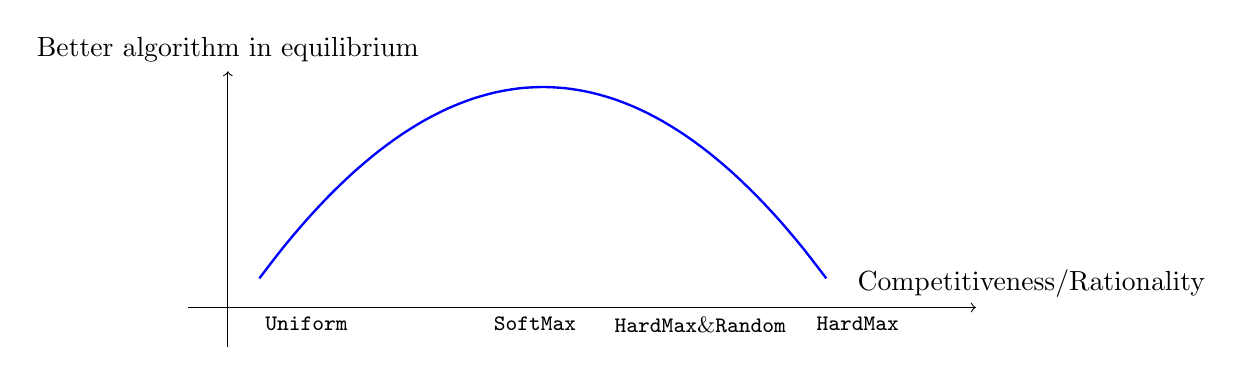
\begin{tikzpicture}[scale=1]
      \draw[->] (-.5,0) -- (9.5,0) node[above] 
        {\qquad\qquad Competitiveness/Rationality};
      \draw[->] (0,-.5) -- (0,3) node[above] {Better algorithm in equilibrium};
      \draw[scale=0.8,domain=0.5:9.5,smooth,variable=\x,blue, line width=0.3mm] plot ({\x},{3.5 - 0.15*(\x - 5)^2});
     \node[below] at (1, 0) {\footnotesize \Uniform};
     \node[below] at (3.9, 0) {\footnotesize \SoftMaxRandom};
     \node[below] at (6, 0) {\footnotesize \HardMaxRandom};
     \node[below] at (8, 0) {\footnotesize \HardMax};
      % \draw[scale=0.5,domain=-3:3,smooth,variable=\y,red]  plot ({\y*\y},{\y});
 \end{tikzpicture}

\caption{The stylized inverted-U relationship in the ``main story".}
\label{fig:inverted-U2}
\end{center}
\end{figure}


\xhdr{Secondary story.}
Let us zoom in on the symmetric  \HardMaxRandom model. \asedit{Competitiveness and rationality within this model are controlled by the baseline probability $\eps_0 = \respF(- 1)$, which goes smoothly between the two extremes of \HardMax ($\eps_0=0$) and the uniform choice ($\eps_0=\tfrac12$). Smaller $\eps_0$ corresponds to increased rationality and increased competitiveness.} For clarity, we assume that principal's utility is the number of agents.

We consider the marginal utility of switching to a better algorithm. Suppose initially both principals use some algorithm \alg, and principal 1 ponders switching to another algorithm \alg' which BIR-dominates \alg. \asedit{We are interested in the marginal utility of this switch. Then:}

\begin{itemize}
\item $\eps_0 = 0$ (\HardMax):~~~~ the marginal utility can be negative if \alg is \DynGreedy.

\item $\eps_0$ near $0$:~~~~ only a small marginal utility can be guaranteed, as it may take a long time for $\alg'$ to ``catch up" with \alg, and hence less time to reap the benefits.

\item ``medium-range" $\eps_0$:~~~~ large marginal utility, as $\alg'$ learns fast and gets most agents.

\item $\eps_0$ near $\tfrac12$:~~~~ small marginal utility, as principal 1 gets most agents for free no matter what.
\end{itemize}
The familiar inverted-U shape is depicted in Figure~\ref{fig:inverted-U3}.



\begin{figure}
\begin{center}
\begin{tikzpicture}[scale=1]
      \draw[->] (-.5,0) -- (9.5,0) node[above]  {$\eps_0$};
      \draw[->] (0,-.5) -- (0,3) node[above] {marginal utility};
      \draw[scale=0.8,domain=0.5:9.5,smooth,variable=\x,blue, line width=0.3mm] plot ({\x},{3.5 - 0.15*(\x - 5)^2});
     \node[below] at (.6, 0) {\footnotesize \Uniform};
     \node[above] at (.5, 0) {\footnotesize 0};
     % \node[below] at (3.9, 0) {\footnotesize \SoftMaxRandom};
     % \node[below] at (6, 0) {\footnotesize \HardMaxRandom};
     \node[below] at (7.5,0) {\footnotesize \HardMax};
     \node[above] at (7.5, 0) {\footnotesize 1/2};
      % \draw[scale=0.5,domain=-3:3,smooth,variable=\y,red]  plot ({\y*\y},{\y});
 \end{tikzpicture}

\caption{The stylized inverted-U relationship from the ``secondary story"}
\label{fig:inverted-U3}
\end{center}
\end{figure}




%%% Local Variables:
%%% mode: latex
%%% TeX-master: "main"
%%% End:


\paragraph{Acknowledgment}{ The authors would like to thank Glen Weyl
  for discussions of related work in economics.  }


% Bibliography
% \bibliographystyle{ACM-Reference-Format}
 \bibliographystyle{plainnat}
\bibliography{bib-abbrv-short,bib-AGT,bib-bandits,bib-slivkins,bib-random,bib-ML}

\appendix

\section{Background on multi-armed bandits}
\label{app:examples}

\newcommand{\ExplorExploit}{\term{ExplorExploit}}
\newcommand{\PhasedExplorExploit}{\term{PhasedExplorExploit}}
\newcommand{\RandomDynGreedy}{\term{RandomDynGreedy}}
\newcommand{\SuccesiveElimination}{\term{SuccesiveElimination}}
\newcommand{\SuccesiveEliminationReset}{\term{SuccesiveEliminationReset}}

This appendix provides some pertinent background on multi-armed
bandits (\emph{MAB}). We discuss \BIR and monotonicity of several MAB algorithms, touching upon: \DynGreedy and \StaticGreedy (Section~\ref{sec:MAB-greedy}), ``naive" MAB algorithms that separate exploration and exploitation (Section~\ref{sec:MAB-naive}), and ``smart" MAB algorithms that combine exploration and exploitation (Section~\ref{sec:MAB-smart}).

As we do throughout the paper, we focus on MAB with i.i.d. rewards and a Bayesian prior; we call it \emph{Bayesian MAB} for brevity.


% For a given mean reward vector $\mu$, the $n$-th step instantaneous regret is
%\begin{align}
%\regret(n\mid\mu) &:= \max_{a\in A} \mu_a - \rew(n\mid\mu),\\
%\regretWC(n)    &:=  \sup_{\text{mean reward vectors $\mu$}} \; \BIR(n\mid \mu).
%\end{align}


\subsection{\DynGreedy and \StaticGreedy}
\label{sec:MAB-greedy}

We provide an example when \DynGreedy and \StaticGreedy have
constant \BIR, and prove monotonicity of \DynGreedy. For the
example, it suffices to consider \emph{deterministic rewards} (for
each action $a$, the realized reward is always equal to the mean
$\mu_a$) and \emph{independent priors} (according to the prior
$\priorMu$, random variables $\mu_1 \LDOTS \mu_K$ are mutually
independent) each of {\em full support}.

%\ascomment{This lemma is just one example. Can we argue that constant \BIR is typical/reasonable?}
%
%
%\begin{lemma}
%There is a problem instance of Bayesian MAB such that \StaticGreedy
%and \DynGreedy have (at least) a constant \BIR for all steps. The
%problem instance has two actions, independent priors, and
%deterministic rewards.
%\end{lemma}
%
%\begin{proof}
%To specify the problem instance, it remains to specify the marginal
%distributions mean rewards $\mu_1$ and $\mu_2$ according to the
%prior. We posit that $\mu_1$ is uniform on the interval $[0, 1]$,
%and $\mu_2$ is uniform on the interval $[\tfrac13,1]$.
%
%Note that
%    $\OPT := \E[\max_{a\in A} \mu_a] =(1/3)(2/3)+(2/3)(7/9)=20/27$.
%%\ascomment{The numbers seem wrong, given the below?}
%This holds since with
%probability $1/3$ we have $\mu_1\leq 1/3$ in which case clearly the
%better arm is 2 with $\E[\mu_2]=2/3$ and with probability $2/3$ we
%have both $\mu_1,\mu_2\in[1/3,1]$ and distributed uniformly each.
%
%\StaticGreedy always recommends action $2$. Since
%$\E[\mu_2]=\tfrac23$, \BIR is $2/27$ in all rounds.
%
%\DynGreedy recommends the first agent action $2$. If $\mu_2 > 2/3$
%For all the following agents it recommends action $2$. Otherwise, it
%recommends agent $2$ action $1$ and for all the following agents it
%recommends the better action. The expectation for agents $t\geq 3$
%is $(1/2)(5/6)+(1/2)((1/2)(1/2)+(1/2)(5/9))=49/72$ and has
%instantaneous regret $13/216$.
%\end{proof}

The following claim is immediate from the definition of the CDF
function
\begin{claim}
Assume independent priors. Let $F_i$ be the CDF of the mean reward
$\mu_i$ of action $a_i\in A$. Then, for any numbers
$z_2>z_1>\E[\mu_2]$ we have
    $\Pr[\text{$\mu_1\leq z_1$ and $\mu_2\geq z_2$}] = F_1(z_1)(1-F_2(z_2)) $.
\end{claim}

%\begin{lemma}
%Let $\priorMu$ be the prior of the means, and assume that it is
%independent for each action, where for arm $i$ it has a mean $
%\E[\mu_i]$ and CDF $F_i$. Then, for any $\E[\mu_2] < z_1<z_2$ we
%have that with probability $F_1(z_1)(1-F_2(z_2))$ that both
%$\mu_1\leq z_1$ and $z_2\leq \mu_2$.
%\end{lemma}

%\begin{corollary}
%Any problem instance of Bayesian MAB for two actions and independent
%priors which are full support and deterministic rewards, with
%constant probability \DynGreedy has a constant \BIR for all steps.
%\end{corollary}


We can now draw an immediate corollary of the above claim

\begin{corollary}
Consider any problem instance of Bayesian MAB with two actions and independent
priors which are full support. Then:
\begin{OneLiners}
\item[(a)] With constant probability, \StaticGreedy  has a constant \BIR for all steps.
\item[(b)] Assuming deterministic rewards, with
constant probability \DynGreedy has a constant \BIR for all steps.
\end{OneLiners}
\end{corollary}

\begin{remark}
A similar result holds for  rewards which are distributed as
Bernoulli random variables. In this case we consider accumulative
reward of an action as a random walk, and use a high probability
variation of the law of iterated logarithms. (Details omitted.)
\end{remark}


Next, we show that \DynGreedy is monotone.

\begin{lemma}\label{dgmono}
\DynGreedy is monotone, in the sense that $\rew(n)$ is non-decreasing.
Further, $\rew(n)$ is strictly increasing for every time step $n$ with $\Pr[a_n\neq a_{n+1}]>0$.
\end{lemma}

\begin{proof}
We prove by induction on $n$ that $\rew(n)\leq \rew(n+1)$ for
\DynGreedy. Let $a_n$ be the random variable recommended at time
$t$, then $\E[\mu_{a_n}| \mI_n ]=\rew(n)$. We can rewrite this as:
\[
\rew(n)=\E_{\mI_n}[\E_{r_n}[\mu_{a_n}|r_n,\mI_n]] =
\E_{\mI_{n+1}}[\mu_{a_n}|\mI_{n+1}]
\]
since $\mI_{n+1}=(\mI_n,r_n)$. At time $n+1$ \DynGreedy will select
an action $a_{n+1}$ such that:
\[
\rew(n+1)=\E[\mu_{a_{n+1}}|\mI_{n+1}]\geq \E[\mu_{a_n}
|\mI_n]=\rew(n)
\]
%
%Now after executing action $a_n$ and observing its reward $r_n$
%there are two possibilities. If $a_n$ is still the best action, then
%its expected reward given the information at time $n$ has not
%changed. On the other hand, if $a_n$ is not the best action anymore,
%then it implies that we recommend a better action. In such a case,
%we increase the expected reward. \ymcomment{need to make this
%formal}
which proves the monotonicity. In cases that $\Pr[a_n\neq
a_{n+1}]>0]$ we have a strict inequality, since with some
probability we select a better action then the realization of $a_n$.
\end{proof}


%%%%%%%%%%%%%%%%%%%%%%%

\subsection{``Naive" MAB algorithms that separate exploration and exploitation}
\label{sec:MAB-naive}


%\ascomment{Nicer to have $\BIR(n)\leq n^{-1/3}$.
%Explore-then-exploit does not have that! So, let's use phases of
%exponentially increasing duration.}

MAB algorithm \ExplorExploit$(m)$ initially explores each action
with $m$ agents and for the remaining $T-|A|m$ agents recommends the
action with the highest observed average. In the explore phase it
assigns a random permutation of the $mK$ recommendations.

\begin{lemma}
%Assume that rewards in the range $[0,1]$.
The \ExplorExploit$(T^{2/3}\log |A|/\delta)$ algorithm has, with
probability $1-\delta$, for any  $n\geq |A|T^{2/3}$ we have
\BIR$(n)=O(T^{-1/3})$. In addition, \ExplorExploit$(m)$ is monotone.
\end{lemma}

\begin{proof}
In the explore phase we we approximate for each action $a\in A$, the
value of $\mu_a$ by $\hat{\mu}_a$. Using the standard Chernoff
bounds we have that with probability $1-\delta$, for every action
$a\in A$ we have $|\mu_a -\hat{\mu}_a| \leq T^{-1/3}$.

Let $a^* = \arg\max_a \mu_a$ and $a^{ee}$ the action that
\ExplorExploit selects in the explore phase after the first
$|A|T^{2/3}$ agents. Since $\hat{\mu}_{a^*} \leq
\hat{\mu}_{a^{ee}}$, this implies that $\mu_{a^*} -
\mu_{a^{ee}}=O(T^{-1/3})$.

To show that \ExplorExploit$(m)$ is monotone, we need to show only
that $\rew(mK) \leq \rew(mK+1)$. This follows since for any $t< mK$
we have $\rew(t)=\rew(t+1)$, since the recommended action is
uniformly distributed for each time $t$. Also, for any $t\geq mK+1$
we have $\rew(t)=\rew(t+1)$ since we are recommending the same
exploration action. The proof that $\rew(mK) \leq \rew(mK+1)$ is the
same as for \DynGreedy in Lemma~\ref{dgmono}.
\end{proof}

We can also have a a phased version which we call
\PhasedExplorExploit$(m_t)$, where time is partition in to phases.
In phase $t$ we have $m_t$ agents and a random subset of $K$ explore
the actions (each action explored by a single agent) and the other
agents exploit. (This implies that we need that $m_t\geq K$ for all
$t$. We also assume that $m_t$ is monotone in $t$.)

\begin{lemma}
Consider the case that $K=2$ and the rewards of the actions are
Bernoulli r.v. with parameter $\mu_i$ and $\Delta=\mu_1-\mu_2$.
Algorithm \PhasedExplorExploit$(m_t)$ is monotone and for $m_t =
\sqrt{t}$ it has $\BIR(n)=O(n^{-1/3}+e^{-O(\Delta^2 n^{2/3})}))$. 
\end{lemma}

\begin{proof}
We first show that it is monotone. Recall that $\mu_1>\mu_2$. Let
$S_i=\sum_{j=1}^t r_{i,j}$ be the sum of the rewards of action $i$
up to phase $t$. We need to show that $\Pr[S_1>S_2]+ (1/2)
\Pr[S_1=S_2]$ is monotonically increasing in $t$. Consider the
random variable $Z=S_1-S_2$. At each phase it increases by $+1$ with
probability $\mu_1(1-\mu_2)$, decreases by $-1$ with probability
$(1-\mu_1)\mu_2$ and otherwise does not change.

Consider the values of $Z$ up to phase $t$. We really care only
about the probability that is shifted from positive to negative and
vice versa.

First, consider the probability that $Z=0$. We can partition it to
$S_1=S_2=r$ events, and let $p(r,r)$ be the probability of this
event. For each such event, we have $p(r,r)\mu_1$ moved to $Z=+1$
and $p(r,r)\mu_2$ moved to $Z=-1$. Since $\mu_1>\mu_2$ we have that
$p(r,r)\mu_1\geq p(r,r)\mu_2$ (note that $p(r,r)$ might be zero, so
we do not have a strict inequality).

Second, consider the probability that $Z=+1$ or $Z=-1$. We can
partition it to $S_1=r+1;S_2=r$ and $S_1=r;S_2=r+1$ events, and let
$p(r+1,r)$ and $p(r,r+1)$ be the probabilities of those events.
%
It is not hard to see that $p(r+1,r)\mu_2=p(r,r+1)\mu_1$.
%
This implies that the probability mass moved from $Z=+1$ to $Z=0$ is
identical to that moved from $Z=-1$ to $Z=0$.

We have showed that $\Pr[S_1>S_2]+ (1/2) \Pr[S_1=S_2]$ and therefore
the expected valued of the exploit action is non-decreasing. Since
we have that the size of the phases are increasing, the $\BIR$ is
strictly increasing between phases and identical within each phase.

We now analyze the $\BIR$ regret. Note that agent $n$ is in phase
$O(n^{2/3})$ and the length of his phase is $O(n^{1/3})$. The $\BIR$
has two parts. The first is due to the exploration, which is at most
$O(n^{-1/3})$. The second is due to the probability that we exploit
the wrong action. This happens with probability $\Pr[S_1<S_2]+ (1/2)
\Pr[S_1=S_2]$ which we can bound using a Chernoff bound by
$e^{-O(\Delta^2n^{2/3})}$, since we explored each action
$O(n^{2/3})$ times.
\end{proof}

\begin{remark}
Actually we have a tradeoff depending on the parameter $m_t$ between
the regret due to exploration and exploitation. (Note that the
monotonicity is always guarantee assuming $m_t$ is monotone.) If we
can set that $m_t = 2^t$ then at time $n$ we have $2/ n$ probability
of an exploit action. For the explore action we are in phase $\log
n$ so the probability of a sub-optimal explore action is
$n^{-O(\Delta^{-2})}$. This should give us
$\BIR(n)=O(n^{-O(\Delta^{-2})})$.
\end{remark}


%MAB algorithm \RandomDynGreedy$(q_t)$for agent $t$ with probability
%$q_t$ selects a random action from $A$ and with probability $1-q_t$
%recommends the best action according to the current posterior
%(similar to \DynGreedy).
%\begin{lemma}
%%Assume that rewards in the range $[0,1]$.
%The algorithm \RandomDynGreedy$(q_t)$, where $q_t=t^{-1/3}$, has,
%with probability $1-\delta$, \BIR$(n)=O(K^{1/2}n^{-1/3}\log
%(K/\delta))$.
%\end{lemma}
%
%\begin{proof}
%At time $n$ we have that with probability $1-\delta/(2K)$, each
%action $a\in A$ was selected at least $n_a=\Theta(n^{2/3}/K)$ times.
%%
%This implies that with probability $1-\delta/(2K)$, for each $a$ we
%have $|\hat{\mu}_a-\mu_a|\leq K^{1/2}n^{-1/3}\log((2K)/\delta)$.
%%
%Therefore, the \BIR is $O(K^{1/2}n^{-1/3}\log((K)/\delta))$
%\end{proof}

%\ascomment{Add: can we modify Phased Explore-then-exploit to make it
%monotone? Perhaps choose exploration rounds u.a.r. within the
%phase?}

%
%\begin{lemma}
%\ExplorExploit$(m)$ is monotone
%\end{lemma}
%
%\begin{proof}
%We need to consider only time $m'=|A|m+1$. For any $n<m'$, we
%clearly have $\rew(n)=\rew(1)$.
%
%Consider two actions $a_1,a_2\in A$, such that $\mu_{a_1} \geq
%\mu_{a_2}$. We claim that the probability that $a_1$ is selected at
%time $m$ to be the exploit action is larger than the probability
%that $a_2$ is selected. This follows since $\hat{\mu}_{a_1}$
%stochastically dominates $\hat{\mu}_{a_2}$, which implies that for
%any threshold $\theta$ we have $\Pr[\hat{\mu}_{a_1}\geq\theta]\geq
%\Pr[\hat{\mu}_{a_2}\geq\theta]$.
%
%After the elimination we consider the expected reward of the
%selected action $\sum_{i\in A} \mu_i q_i$, where $q_i$ is the
%probability that action $i$ was selected for the exploit phase. We
%have that $q_i \geq q_{i+1}$, from the stochastic dominance.
%
%The sum $\sum_{i\in A} \mu_i q_i$ with $q_i \geq q_{i+1}$ and
%$\sum_i q_i=1$ is minimized by setting $q_i=1/|A|$. (We can see that
%if there are $q_i\neq 1/|A|$, then there are two $q_{i}> q_{i+1}$,
%and one can see that setting both to $(q_{i}+ q_{i+1})/2$ decreases
%the value.) Therefore we have that the $\rew(m')\geq\rew(m'-1)$.
%\end{proof}


\subsection{``Smart" MAB algorithms that combine exploration and exploitation}
\label{sec:MAB-smart}


%MAB algorithm \SuccesiveElimination holds a set of action
%$A_s\subset A$ which are called {\em surviving actions} and for
%agent $t$ selects a random action from $A_s$. Let $n_{i,t}$ be the
%number of times action $i$ has been selected up to time $t$, and
%$\hat{\mu}_{i,t}$ be the average of the rewards of action $i$ up to
%time $t$ and $\hat{\mu}^*=\max_i \hat{\mu}_{i,t}$. We eliminate
%action $i$ at time $t$, i.e., delete it from $A_s$, if
%$\hat{\mu}_t^*-\hat{\mu}_{i,t} > \log(T/\delta)/\sqrt{n/K}$.
%
%\begin{lemma}
%Assume that the prior is independent and if $\mu_i\geq \mu_j$ then
%$r_i$ stochastically dominates $r_j$.
%%
%The algorithm \SuccesiveElimination, has, with probability
%$1-\delta$, \BIR$(n)=O(\log(T/\delta)/\sqrt{n/K})$.
%\end{lemma}

%\begin{proof}
%Let the best action be $a^*=\arg\max_a \mu_a$. With probability
%$1-\delta$ at any time $n$ we have that for any action $i\in A_s$
%that $|\hat{\mu}_i -\mu_i|\leq \log(T/\delta)/\sqrt{n/K}$, and
%$a^*\in A_s$. This implies that any action $a$ such
%$\mu_{a^*}-\mu_{a}> 3\log(T/\delta)/\sqrt{n/K}$ is eliminated.
%Therefore, any action in $A_s$ has \BIR$(n)$ of at most
%$O(\log(T/\delta)/\sqrt{n/K})$. \ymcomment{should we get the
%constant right?}
%\end{proof}




%\ascomment{Add: Successive Elimination is monotone (or a simple
%modification thereof).}
%
%\begin{lemma}
%\SuccesiveElimination is monotone
%\end{lemma}
%
%\begin{proof}
%We will first show that for any two actions $a_1,a_2\in A$ that if
%$\mu_{a_1} \geq \mu_{a_2}$ then at any time $t$ we have that the
%probability that $a_1$ is eliminated is smaller than the probability
%that $a_2$ is eliminated, i.e., $\Pr[a_1 \not\in A_{s,t+1}| a_1\in
%A_{s,t} ]\geq \Pr[ a_2 \not\in A_{s,t+1}| a_2\in A_{s,t}]$.
%
%We first show that given this statement, the lemma holds and
%\SuccesiveElimination is monotone. Consider $\rew(t)$ versus
%$\rew(t+1)$. If the elimination probabilities would have been
%identical then we would have $\rew(t)=\rew(t+1)$. Consider the top
%two actions, and consider the elimination process in two phases,
%firs we eliminate both with the same probability, and hence the
%reward is unchanged, and then we eliminate only the second, which
%implies that we increase the the reward. The claim about the
%elimination probabilities rules out the case that the elimination
%probability of the best action is higher than then of the the second
%best. Therefore, overall the reward can only increase.
%
%
%We now need to prove the claim. Since $\mu_{a_1}\geq \mu_{a_2}$ and
%they use the same parametric family $\psi_a(\cdot)$ then
%$\hat{\mu}_{a_1}$ stochastically dominates $\hat{\mu}_{a_2}$. We
%actually need to show that $\hat{\mu}_{a_1}$ stochastically
%dominates $\hat{\mu}_{a_2}$ given that $a_1,a_2\in A_{s,t}$. If this
%holds, then the claim about the elimination would be immediate,
%since for any threshold $\theta$ we have $\Pr[\hat{\mu}_{a_1,t} <
%\theta |a_1\in A_{s,t}] \leq \Pr[\hat{\mu}_{a_2,t} < \theta |a_2\in
%A_{s,t}] $. By setting $\theta=\hat{\mu}^*-
%\log(T/\delta)/\sqrt{n/K}$ we derive the lemma.
%
%We now need to prove the claim. We first show that
%$\E[\hat{\mu}_{a_1}-\hat{\mu}_{a_2} | a_1,a_2\in A_s]\geq 0$ which
%is equivalent to $\E[\hat{\mu}_{a_1}-\hat{\mu}_{a_2} |
%\hat{\mu}_{a_1},\hat{\mu}_{a_2}\geq \hat{\mu}^*-\theta]\geq 0$ where
%$\theta$ is the threshold used in \SuccesiveElimination. Since
%action $a_1$ has a high expectation than $a_2$ it holds (at least
%for Bernoulli r.v.).
%
%
%[[OLD]]
%
% Clearly, for any actions $a\in A$ we have that $\Pr[a \in
%A_s]$ decreases with time. In addition, we have that with
%probability $1-\delta$ for every time $t$ we have $a^*\in A_s$.
%
%If $\mu_{a_1} \geq \mu_{a_2}$ then at any time $t$ we have
%$\Pr[a_1\in A_s]\geq \Pr[a_2\in A_s]$.
%
%
%We probably need to show that if $\mu_{a_1} \geq \mu_{a_2}$ then at
%any time $t$ we have that the probability that $a_1$ is eliminated
%is smaller than the probability that $a_2$ is eliminated, i.e.,
%$\Pr[a_1\in A_{s,t}, a_1 \not\in A_{s,t+1}]\geq \Pr[a_2\in A_s, a_2
%\not\in A_{s,t+1}]$.
%\end{proof}




%\ymcomment{Here is a simple modification of Successive-Elimination}



MAB algorithm \SuccesiveEliminationReset works as follows. It keeps
a set of surviving actions $A_s\subseteq A$, where initially
$A_s=A$. The agents are partition into phases, where each phase is a
random permutation of the non-eliminated actions.
% Initially, we select actions at random. Let $n_{i,t}$
%be the number of times action $i$ has been selected up to time $t$,
Let $\hat{\mu}_{i,t}$ be the average of the rewards of action $i$ up
to phase $t$ and $\hat{\mu}^*=\max_i \hat{\mu}_{i,t}$. We eliminate
action $i$ at the end of phase $t$, i.e., delete it from $A_s$, if
$\hat{\mu}_t^*-\hat{\mu}_{i,t} > \log(T/\delta)/\sqrt{t}$.
%So far identical to \SuccesiveElimination, the difference is how we
%continue after elimination.
In \SuccesiveEliminationReset we simply reset the algorithm with
$A=A_s-A_{e,t}$, where $A_{e,t}$ is the set of eliminated actions
after phase $t$. Namely, we restart $\hat{\mu}_{i,t}$ and ignore the
old rewards before the elimination.

\begin{lemma}
%
The algorithm \SuccesiveEliminationReset, has, with probability
$1-\delta$, \BIR$(n)=O(\log(T/\delta)/\sqrt{n/K})$.
\end{lemma}

\begin{proof}
Let the best action be $a^*=\arg\max_a \mu_a$. With probability
$1-\delta$ at any time $n$ we have that for any action $i\in A_s$
that $|\hat{\mu}_i -\mu_i|\leq \log(T/\delta)/\sqrt{n/K}$, and
$a^*\in A_s$. This implies that any action $a$ such
$\mu_{a^*}-\mu_{a}> 3\log(T/\delta)/\sqrt{n/K}$ is eliminated.
Therefore, any action in $A_s$ has \BIR$(n)$ of at most
$6\log(T/\delta)/\sqrt{n/K}$.
\end{proof}

\begin{lemma}
Assume that if $\mu_i\geq \mu_j$ then the rewards $r_i$
stochastically dominates the rewards $r_j$.
%
Then, \SuccesiveEliminationReset is monotone
\end{lemma}

\begin{proof}
Consider the first time $T$ an action is eliminated, and let
$T=\tau$ be a realized value of $T$. Then, clearly for $n<\tau$ we
have $\rew(n)=\rew(1)$ .

Consider two actions $a_1,a_2\in A$, such that $\mu_{a_1} \geq
\mu_{a_2}$. At time $T=\tau$, the probability that  $a_1$ is
eliminated is smaller than the probability that $a_2$ is eliminated.
This follows since $\hat{\mu}_{a_1}$ stochastically dominates
$\hat{\mu}_{a_2}$, which implies that for any threshold $\theta$ we
have $\Pr[\hat{\mu}_{a_1}\geq\theta]\geq
\Pr[\hat{\mu}_{a_2}\geq\theta]$.

After the elimination we consider the expected reward of the
eliminated action $\sum_{i\in A} \mu_i q_i$, where $q_i$ is the
probability that action $i$ was eliminated in time $T=\tau$. We have
that $q_i \leq q_{i+1}$, from the probabilities of elimination.

The sum $\sum_{i\in A} \mu_i q_i$ with $q_i \leq q_{i+1}$ and
$\sum_i q_i=1$ is maximized by setting $q_i=1/|A|$. (We can see that
if there are $q_i\neq 1/|A|$, then there are two $q_{i}< q_{i+1}$,
and one can see that setting both to $(q_{i}+ q_{i+1})/2$ increases
the value.) Therefore we have that the $\rew(\tau)\geq\rew(\tau-1)$.

Now we can continue by induction. For the induction, we can show the
property for {\em any} remaining set of at most $k-1$ actions. The
main issue is that \SuccesiveEliminationReset restarts from scratch,
so we can use induction.
\end{proof}







\end{document} 